% Manuscript draft v12 (restructured) aligned to the supplied ICLR/IPM examples.

\documentclass[10pt]{article}

% --- Packages ---
\usepackage[T1]{fontenc}
\usepackage[utf8]{inputenc}
\usepackage[letterpaper,margin=0.74in]{geometry}
\usepackage{setspace}
\setstretch{1.0}

\usepackage{natbib}
\usepackage{graphicx}
\graphicspath{{./}{../}}
\usepackage{booktabs}
\usepackage{tabularx}
\usepackage{array}
\usepackage{ragged2e}
\newcolumntype{Y}{>{\RaggedRight\arraybackslash}X}
\newcolumntype{C}{>{\centering\arraybackslash}p{0.12\textwidth}}
\newcolumntype{L}[1]{>{\RaggedRight\arraybackslash}p{#1}}
\usepackage{amsmath,amssymb}
\usepackage{hyperref}
\usepackage{xurl}
\hypersetup{colorlinks=true,linkcolor=black,citecolor=blue,urlcolor=blue}
\usepackage[activate={true,nocompatibility},expansion=false,protrusion=true]{microtype}
\usepackage{float}
\usepackage{titlesec}
\usepackage[font=footnotesize,labelfont=bf]{caption}
\usepackage{enumitem}

% Single-spaced, paper-like typography: no draft line numbers or paragraph gaps.
\setlength{\parindent}{1.15em}
\setlength{\parskip}{0pt plus 0.1pt}
\setlength{\textfloatsep}{7pt plus 2pt minus 2pt}
\setlength{\floatsep}{6pt plus 2pt minus 2pt}
\setlength{\intextsep}{7pt plus 2pt minus 2pt}
\setlength{\abovecaptionskip}{3pt}
\setlength{\belowcaptionskip}{0pt}
\setlist[itemize]{leftmargin=1.4em,itemsep=1pt,topsep=2pt,parsep=0pt}
\setlist[enumerate]{leftmargin=1.6em,itemsep=1pt,topsep=2pt,parsep=0pt}
\titleformat{\section}{\large\bfseries}{\thesection.}{0.55em}{}
\titleformat{\subsection}{\normalsize\bfseries}{\thesubsection.}{0.55em}{}
\titleformat{\paragraph}[runin]{\bfseries}{\theparagraph}{0.5em}{}[]
\titlespacing*{\section}{0pt}{1.05ex plus .25ex}{0.55ex}
\titlespacing*{\subsection}{0pt}{0.85ex plus .2ex}{0.3ex}
\titlespacing*{\paragraph}{0pt}{0.7ex plus .2ex}{0.65em}
\captionsetup{font=footnotesize,labelfont=bf}

% Allow slightly more flexible spacing to handle math-heavy paragraphs gracefully.
\sloppy
\emergencystretch=2em

\renewenvironment{abstract}{%
  \vspace{0.15em}
  \begin{center}\small\bfseries A B S T R A C T\end{center}
  \vspace{-0.9em}
  \small\noindent
}{\par\vspace{0.55em}}

\newcommand{\compacttitle}{%
  \vspace*{-1.25em}
  \begin{flushleft}
  {\LARGE\bfseries Recurrent Connection Topology Supports Reactive Control through Propagation Dynamics in Fixed-Weight Spiking Neural Networks\par}
  \vspace{0.55em}
  {\normalsize Xuewei Li$^{1,\dagger,*}$, Bowen Zhao$^{2,\dagger}$, and Guangxu Mei$^{3}$\par}
  \vspace{0.2em}
  {\small $^1$SYNTHESIS ELECTRONIC TECHNOLOGY Co., Ltd.\\[-0.03em]
  $^2$Shandong University of Science and Technology\\[-0.03em]
  $^3$Shandong University\par}
  \vspace{0.15em}
  {\small $^\dagger$Co-first authors. \quad $^*$Corresponding author.\par}
  \end{flushleft}
  \vspace{0.35em}
  \hrule height 0.4pt
  \vspace{0.65em}
}

\begin{document}

\compacttitle
\begin{abstract}
Neural computation is commonly attributed to the optimization of synaptic
weights, the principle underlying the deep-learning paradigm. Evidence from
connectomics, however, shows that circuit connectivity is highly structured,
raising the possibility that computation can rely substantially on signal
propagation through this structure rather than on precise per-synapse weight
values alone. Here we test this
idea under a strict fixed-weight setting: every synaptic weight is determined by
$W[i,j]=A[i,j]\times\text{type}[i]\times\mathit{weight\_scale}$, where the
excitatory or inhibitory type of each neuron is assigned in advance and then
frozen, and a genetic algorithm evolves only the binary adjacency matrix $A$.
Across discrete control tasks and single-topology continuous-control
proof-of-concept experiments, this topology-only search produces viable
reactive policies in the tested benchmark regime. In an aligned CartPole
control experiment, whose endpoint is bounded by the 500-step ceiling, it does
not produce a detectable performance loss relative to a same-size network whose
individual weights are co-evolved, while reducing continuous synaptic-weight
degrees of freedom by four orders of magnitude; on MountainCar, the
corresponding uncertainty interval is much wider. A LunarLander-v3 headroom
audit removes the CartPole ceiling but does not support strict 10\% TOST
equivalence: topology-only evolution shows no systematic disadvantage relative
to independent-weight co-evolution in this sample, but the supported equivalence
margin is broader than the pre-specified primary margin. We therefore treat the
weight-comparison result as a bounded no-systematic-disadvantage finding, not as
a formal equivalence claim. Mechanistic analyses are consistent with temporal
iterative propagation while acknowledging remaining confounds: reducing the
number of internal propagation passes sharply reduces performance, and hidden
activity retains linearly decodable traces of recent inputs over task-matched
timescales. A
non-spiking rate-substitution control on the same evolved topology fails to
recover CartPole performance without re-evolution. Across five discrete task
configurations, independently evolved topologies show configuration-separable
structural fingerprints (leave-one-out KNN accuracy 94.0\%), but an explicit
metadata audit shows that this fingerprint is partly confounded by task-specific
network size and input/output dimensions. The continuous-control extension remains a
proof of concept: a single Hopper-v4 topology reaches 48\% of a 1M-step PPO
reference with a single global weight-scale parameter, but the method remains
below PPO and does not yet reach proficiency on higher-dimensional action
spaces. We treat these negative cases as boundaries of the present
instantiation---small 64--128-neuron networks searched by a genetic
algorithm---rather than as general limits of fixed-weight structure. For
reactive control and short-timescale temporal integration, these results
provide evidence that binary recurrent structure, together with a compatible
global dynamical scale, can support control policies under fixed per-synapse
weights, while indicating where this regime currently breaks down.
\end{abstract}

\section{Introduction}

Understanding how neural circuits give rise to behavior is a central question
in computational neuroscience. In artificial neural network research, the
prevailing answer is that behavior is determined by the precise numerical
configuration of synaptic weights---the view embodied by the deep-learning
paradigm, whose core operation is the gradient-based optimization of large
numbers of floating-point weights. Evidence from biological neuroscience,
however, points to a complementary possibility. The nematode \textit{C.\ elegans}
produces a rich repertoire of sensorimotor behaviors from an essentially fixed
302-neuron connectome \citep{white1986,cook2019,varshney2011}, and recent
whole-brain reconstructions of \textit{Drosophila} \citep{dorkenwald2024,scheffer2020,eichler2017}
show highly structured anatomical wiring, with identifiable topological
organization (for example, the sparse coding of the mushroom body and the ring
organization of the fan-shaped body) visible at the circuit level. Comparative
work further associates
increases in behavioral complexity along phylogeny with specific changes in
neural organization rather than with neuron count alone \citep{striedter2005,cisek2019}.
Together these observations motivate a complementary view: signal propagation
through connection topology may carry a substantial part of circuit computation
alongside synaptic tuning.

Artificial neural network research offers an indirect echo. The lottery ticket
hypothesis \citep{frankle2019,frankle2020} shows that large randomly
initialized networks contain sparse subnetworks that, trained in isolation,
match the full network, and that some subnetworks perform reasonably with no
training at all \citep{ramanujan2020}. Supermask work further shows that binary
masks and sign patterns over untrained weights can carry nontrivial function
\citep{zhou2019}. Weight-agnostic neural networks evolve architectures that can
perform under shared-weight settings \citep{gaier2019}, including spiking
circuit extensions \citep{anwar2021}, and recent work on evolving recurrent
spiking connectivity searches sparse boolean RSNN connectivity for locomotion
tasks \citep{wang2023}. Reservoir computing
\citep{jaeger2001,maass2002,lukosevicius2009,tanaka2019} fixes the recurrent
layer entirely and trains only a readout, remaining competitive on a range of
temporal tasks; and fixed spiking networks are attractive on neuromorphic
hardware \citep{davies2018,roy2019}. These settings make clear that
connectivity is a powerful computational variable. Our narrower question is
whether reactive control can still be supported when per-synapse trainable
magnitudes are removed, the E/I sign scaffold and global scale are fixed, and
the action readout has no trained weights.

To isolate this structural contribution, we therefore ask a sharper
control-variable question: \emph{when independently tunable per-synapse weights
are removed, can a binary recurrent topology under a fixed global weight scale
still support a control policy?} We fix every nonzero
synaptic magnitude to a single global
scale---the weight from neuron $i$ to $j$ is
$W[i,j]=A[i,j]\times\text{type}[i]\times\mathit{weight\_scale}$, where each
neuron's excitatory or inhibitory type is assigned before evolution and then
frozen and the sign of every outgoing weight follows that type---and we apply a
variation--selection search (a genetic algorithm) only to the binary adjacency
matrix $A\in\{0,1\}^{N\times N}$. This reduces the optimization target from the
$O(N^2)$ continuous weights of a conventional network to $N^2$ binary variables
under a fixed global scale, so that successful control cannot be attributed to
independently tuned synaptic weights, but must arise from the binary connection
pattern together with the fixed dynamical rules. This setup should be read as
an engineering stress test of structure--function coupling under fixed
dynamics, not as a model of how biological connectomes form. Throughout,
``topology-only'' refers to the degrees of freedom optimized by the genetic
algorithm; it does not mean that the controller lacks architectural priors such
as the E/I scaffold, global scale, readout rule, network size, or
$T_\text{steps}$ schedule.

Within this setting we examine two questions. First, in CartPole, MountainCar,
and a LunarLander headroom audit, we ask whether topology-only evolution can
reach the performance range of same-size networks whose weights are free to
co-evolve, and how the CartPole case compares with established baselines (NEAT
and PPO). Second, we examine
\emph{how} a fixed-weight network supports control when it succeeds: whether function depends on the enrichment of local
connection motifs or on temporal propagation through the evolved graph, and
whether recent input history is reflected in the internal propagation dynamics. We
restrict our claims to reactive control and short-timescale temporal
integration. We also map the boundary of the approach---the task types on which
it fails and the action dimensionality at which it becomes less effective at the present
network scale---since this boundary is itself an informative result that helps
delineate the regime in which binary connection structure together with a
compatible global scale can be sufficient in these benchmark settings.

We make the following contributions:
\begin{itemize}
\item We introduce a fixed-weight spiking controller in which individual
synaptic weights are not learned: each weight is determined by a binary
adjacency matrix, a frozen excitatory/inhibitory type assignment, and a fixed
global weight scale.
\item We show that, under aligned CartPole and MountainCar controls, evolving
only the binary topology does not produce a detectable performance loss relative
to co-evolving a global scale or independent per-synapse weights. A
LunarLander-v3 headroom audit further removes the CartPole ceiling: TO is not
systematically below TI in that sample, but the pre-specified 10\% TOST
equivalence test fails. These confidence-interval and TOST sensitivity
boundaries prevent the comparison from being read as unrestricted equivalence;
in a separate CartPole positioning audit, the method falls within the same
ceiling regime as NEAT and PPO without any independently tuned per-synapse
weights.
\item We provide converging but still partly correlational evidence---$T_\text{steps}$ ablation, input-history
decoding, intermediate-state perturbation, and history-dependent spike
timing---pointing to temporal iterative propagation through the evolved graph as
a candidate mechanism, rather than local connection-motif enrichment or precise
hidden membrane values alone; a non-spiking rate-substitution control on the
same topology does not reproduce the CartPole policy without re-evolution.
\item We characterize task/configuration-specific structural fingerprints,
explicitly audit their architecture-size confounding, report single-topology
continuous-control proof-of-concepts, and identify boundary cases, including
working-memory tasks, cross-configuration transfer, and higher-dimensional
action spaces.
\end{itemize}

\section{Related Work}

\subsection{Topology, sparsity, and weight-free subnetworks}

A line of work in deep learning has shown that much of a trained network's
function can be located in its connectivity rather than in the precise values
of its weights. The lottery ticket hypothesis \citep{frankle2019,frankle2020}
demonstrates that dense networks contain sparse subnetworks whose connectivity,
when trained in isolation from the original initialization, matches the full
network. \citet{ramanujan2020} push this further, showing that within a
sufficiently large randomly weighted network one can find subnetworks that
perform well with no weight training at all, purely by selecting which
connections to keep; related supermask results emphasize that binary masks and
sign patterns can encode function even before ordinary weight training
\citep{zhou2019}. Weight-agnostic neural networks \citep{gaier2019}, including
spiking circuit extensions \citep{anwar2021}, evolve architectures that can
function across shared weight values without learning independent per-edge
weights. These results indicate that connection structure
carries substantial functional information. In most of these studies, however,
the selected subnetwork still inherits a particular configuration of real-valued
weights; in weight-agnostic networks, architectures are evaluated with respect
to shared continuous weight values. Our setting differs in that per-synapse
weight values are removed entirely---all nonzero magnitudes share a single fixed
global scale---so that the only quantity searched is the binary connection
pattern itself.

\subsection{Fixed-weight recurrent networks and reservoir computing}

Reservoir computing fixes a recurrent network and trains only a linear readout.
Echo state networks \citep{jaeger2001} and liquid state machines
\citep{maass2002}, surveyed by \citet{lukosevicius2009} and \citet{tanaka2019},
show that a fixed random recurrent substrate can project inputs into a
high-dimensional dynamical space rich enough for a simple readout to solve
temporal tasks. This establishes that useful temporal computation can arise
from fixed recurrent connectivity. Reservoir computing nonetheless still learns
the readout weights, so the trained readout, rather than the fixed recurrent
structure, carries the task-specific mapping. Related ideas appear in spiking
models \citep{maass1997,gerstner2014} and in attractor networks
\citep{hopfield1982}, where fixed connectivity supports stable computational
states. In contrast to these, the network studied here has no trained readout:
the action is read directly from output spike counts under a fixed rule, so any
task-specific function must reside in the evolved connection topology together
with the fixed dynamics.

\subsection{Neuroevolution and topology search}

Evolving network structure has a long history in neuroevolution. NEAT
\citep{stanley2002} incrementally complexifies network topology while
simultaneously evolving connection weights, and HyperNEAT \citep{stanley2009}
evolves a generative encoding of large-scale connectivity. These methods
establish that variation--selection search over structure can produce competent
controllers, and they provide a natural point of comparison for our work. The
defining feature of NEAT-style methods, however, is the joint evolution of
topology and weights, which leaves the contribution of structure entangled with
that of the co-evolved weights. We instead isolate structure by searching only
the binary adjacency matrix with a genetic algorithm \citep{holland1992,eiben2015}
while holding all weight magnitudes at a single fixed global scale, and we use
NEAT as one of our positioning baselines on CartPole.

The closest spiking-neuroevolution precedent is the evolution of recurrent
spiking connectivity with sparse boolean connection variables
\citep{wang2023}. That line of work demonstrates that evolved RSNN connectivity
can support locomotion under neuromorphic-friendly constraints, and is therefore
a direct point of comparison rather than background only. Our contribution is a
stricter control-variable variant: neuron signs follow a frozen Dale-like
scaffold, all nonzero synapses share one global magnitude, the readout is a
fixed spike-count rule, and the empirical focus is not benchmark superiority but
the audit of what binary recurrent topology can and cannot support once
independently tunable per-synapse weights are removed. Table~\ref{tab:close-work}
summarizes this positioning.

\begin{table}[H]
\centering
\footnotesize
\begin{tabularx}{\textwidth}{L{0.17\textwidth} L{0.10\textwidth} L{0.10\textwidth} L{0.18\textwidth} Y}
\toprule
\textbf{Work} & \textbf{Spiking} & \textbf{Recurrent} & \textbf{Searched weights} & \textbf{Main distinction from this paper} \\
\midrule
WANN / spiking WANN \citep{gaier2019,anwar2021} & Sometimes & Optional & Shared values & Evolves architectures or motifs evaluated across shared weights; not a fixed Dale-sign recurrent SNN with one global magnitude and direct spike-count readout. \\
Supermask subnetworks \citep{ramanujan2020,zhou2019} & No & No & Masks/signs over initialized weights & Searches subnetworks inside large random or trained-weight spaces rather than small recurrent controllers evolved from scratch. \\
Evolving RSNN connectivity \citep{wang2023} & Yes & Yes & Boolean connectivity & Closest prior work; our variant fixes Dale signs and one global magnitude, removes learned readout weights, and emphasizes mechanism/boundary audits under topology-only search. \\
This paper & Yes & Yes & No independent per-edge magnitudes & Binary adjacency is the only GA-optimized variable; all other dynamics/readout choices are fixed design priors. \\
\bottomrule
\end{tabularx}
\caption{Positioning against close work on weight-free subnetworks and evolved spiking connectivity. The table is intended to delimit the control-variable claim rather than to assert benchmark dominance.}
\label{tab:close-work}
\end{table}

\subsection{Connectome-inspired neural computation}

Connectomics provides the biological motivation for asking what connection
structure can support on its own. The complete wiring diagram of
\textit{C.\ elegans} \citep{white1986,varshney2011,cook2019} and recent
large-scale reconstructions of the \textit{Drosophila} brain
\citep{eichler2017,scheffer2020,dorkenwald2024} show that circuit connectivity
is highly structured and anatomically organized; comparative neuroscience
further associates behavioral complexity with neural organization rather than
neuron count alone
\citep{striedter2005,cisek2019}. Two organizing principles of biological
circuits inform our model: Dale's principle, under which a neuron's outgoing
synapses share a consistent sign \citep{eccles1976,strata1999}, and the characteristic
excitatory/inhibitory composition of cortical circuits
\citep{markram2004,harris2015}. We adopt both as fixed, non-optimized
constraints. Recent connectome-based embodied modeling provides a complementary
computational example: a whole-brain graph model whose static structure follows
the adult \textit{Drosophila} connectome has been used to control a
biomechanical fly body across locomotion tasks and to outperform rewired and
random graph controls \citep{jin2026}. Separately, fixed-topology spiking
networks are central to neuromorphic computing
\citep{maass1997,davies2018,roy2019,schuman2017}, where efficiency derives from
sparse, event-driven connectivity; our results speak to what such
fixed-connectivity systems can compute before any on-chip weight adaptation.

\section{Method}

\subsection{Problem formulation}
\label{sec:problem}

We study whether a binary recurrent connection topology, evaluated under fixed
dynamics and a single global weight scale, can support a reactive control
policy. A controller is a recurrent spiking network of $N$ neurons whose synaptic
weight from neuron $i$ to neuron $j$ is given by
\begin{equation}
W[i,j] = A[i,j] \times \text{type}[i] \times \mathit{weight\_scale},
\label{eq:weight}
\end{equation}
where $A \in \{0,1\}^{N \times N}$ is a binary adjacency matrix,
$\text{type}[i] \in \{+1,-1\}$ fixes neuron $i$ as excitatory or inhibitory, and
$\mathit{weight\_scale}$ is a single global scalar. Three quantities are fixed
before topology search: the neuron-type vector $\text{type}$ (assigned once per
independent seed at random, with the inhibitory fraction held at $30\%$), the
dynamical rule (Section~\ref{sec:controller}), and the global scale. In the five
discrete topology-only experiments the scale is fixed at $0.6$; this value was
chosen before the TO/TG/TI comparison as the default dynamical scale used in the
existence, mechanism, and cross-task experiments, and is not reselected per
seed. The continuous proof-of-concept experiments use fixed task-specified
scales (Pendulum $0.6$ and standard-gravity Hopper $0.5$), and the scale is
retuned only in explicit adaptation analyses. The genetic algorithm searches
only the binary adjacency matrix $A$. Consequently the optimization reduces the
$O(N^2)$ continuous weights of a conventional network to $N^2$ binary variables
under a fixed global scale for a given experiment, and any successful control
cannot be attributed to independently tuned per-synapse weights or to an
implicitly optimized type assignment, but must arise from the binary connection
pattern together with the fixed type scaffold and dynamical rules. Because the
type vector varies across independent seeds, the CartPole result that $19/20$
topology-only seeds reach criterion also indicates that success is not tied to a
single lucky E/I layout. We later relax two of these constraints as explicit
controls---co-evolving the global scale, and co-evolving independent per-synapse
weights---to quantify how much, if anything, weight freedom adds
(Section~\ref{sec:protocol}).

\subsection{Fixed-weight spiking neural controller}
\label{sec:controller}

The $N$ neurons are partitioned into input ($n_\text{in}$), hidden
($n_\text{hidden}$), and output ($n_\text{out}$) populations. The total network
size $N$ ranges from $64$ to $128$ depending on the task, with
$n_\text{hidden} = N - n_\text{in} - n_\text{out}$
(Section~\ref{sec:protocol}). The input size follows the half-wave-rectified
encoding, $n_\text{in} = 2 \times (\text{state dimension})$, since each state
dimension is split into a positive and a negative channel. Each neuron is
assigned a fixed type
$\text{type}[i] \in \{+1,-1\}$ before evolution: an excitatory neuron ($+1$) has
positive-sign outgoing weights and an inhibitory neuron ($-1$) negative-sign
outgoing weights, following Dale's principle \citep{eccles1976,strata1999}. The inhibitory
fraction is held at $30\%$ across all tasks, of the same order as the
excitatory/inhibitory ratio of mammalian cortex \citep{markram2004}. Both the
type vector and the inhibitory fraction are frozen and are not degrees of
freedom under search; under Equation~\ref{eq:weight} all outgoing synapses of a
neuron therefore share a single magnitude and sign, and the presence or absence
of each connection is the only quantity searched.

Neurons follow leaky integrate-and-fire dynamics \citep{gerstner2014}. The
membrane potential $v$ updates as
\begin{equation}
v \leftarrow v\left(1 - \frac{\Delta t}{\tau}\right) + \text{spikes}\cdot W + \frac{\Delta t}{\tau}\,\big(I_\text{ext}\odot m_\text{in}\big),
\label{eq:lif}
\end{equation}
with $\tau = 5.0~\text{ms}$, $\Delta t = 1.0~\text{ms}$, a firing threshold of
$0.8$, and reset to $0$ after a spike. The external drive is injected only into
the input population: $m_\text{in}$ is a binary mask selecting input neurons, and
$I_\text{ext}$ is the half-wave-rectified state (each state dimension split into
a positive and a negative channel). For discrete-action tasks the action is selected by an argmax
over the output spike counts accumulated across $T_\text{steps}$ internal
forward passes; the continuous-action readout is described in
Section~\ref{sec:decoding}. No weights are learned at any point: there is no
gradient descent, no Hebbian update, and no weight adaptation during inference.
Membrane potentials are initialized to zero at the beginning of each episode and
then carried across environment steps within that episode; a decision therefore
uses both the current observation and the network state left by previous
observations.

\subsection{Topology-only genetic evolution}
\label{sec:evolution}

We search the binary adjacency matrix $A$ with a genetic algorithm
\citep{holland1992,eiben2015}, an engineering counterpart of variation--selection
search rather than a simulation of biological evolution: each generation forms a
new population of topologies by variation and selection, moving through the
$2^{N^2}$ space of possible connection patterns toward functional solutions. The
search acts only on $A$; all other components are shared and fixed within each
experiment: the frozen type scaffold and Dale sign rule, the task-specified
global scale (set to $0.6$ for the five discrete tasks), the leaky
integrate-and-fire dynamics of Equation~\ref{eq:lif}, and the absence of any
learning during inference. Within
each generation, elitism retains the top individuals unchanged, mutation applies
random bit flips to $A$, and fitness is computed by a \emph{task-specific} fitness
function during evolution (the per-task score/shaping defined by each
environment), which is kept separate from the protocol-independent strict
$20$-episode evaluation used for all reported comparisons
(Section~\ref{sec:protocol}). At no point does gradient descent, Hebbian
learning, or weight update occur; after evolution the topology is frozen and
inference begins.

Table~\ref{tab:evo-config} lists the per-task network configuration. For the
multi-task existence experiment, all five discrete tasks use population $80$,
$16$ elites, mutation rate $0.03$, and an upper budget of $400$ generations with
early stopping at the task-specific proficiency threshold. The number of evaluation
episodes per genome during evolution is task-specific (10--20 episodes for the
standard Gym-style tasks and 10 episodes for the custom visual-game tasks). The
weight-contribution controls (TO/TG/TI) use the same GA budget but fix the network
size to $128$ neurons for CartPole, MountainCar, and the LunarLander headroom
audit, as specified below.

\begin{table}[H]
\centering
\small
\caption{Per-task network and GA configuration. Input size follows half-wave
rectification ($n_\text{in}=2\times$ state dimension);
$n_\text{hidden}=N-n_\text{in}-n_\text{out}$. The five primary discrete tasks use
population $80$, $16$ elites, mutation rate $0.03$, fixed scale $0.6$, and early
stopping within an upper budget of $400$ generations. LunarLander is an
additional TO/TG/TI headroom audit with the same upper budget and no early
stopping. Pendulum (scale $0.6$) and Hopper (standard-gravity scale $0.5$) are
single-topology continuous-control proof-of-concept runs.}
\label{tab:evo-config}
\begin{tabular}{@{}lccccc@{}}
\toprule
\textbf{Task} & \textbf{State dim} & $\mathbf{n_\text{in}}$ & $\mathbf{n_\text{out}}$ & $\mathbf{N}$ & \textbf{Pop / Max gen} \\
\midrule
CartPole-v1        & 4  & 8  & 2 & 128 & 80 / 400 \\
MountainCar-v0     & 2  & 4  & 3 & 64  & 80 / 400 \\
LunarLander-v3 (headroom audit) & 8 & 16 & 4 & 128 & 80 / 400 \\
Acrobot-v1         & 6  & 12 & 3 & 128 & 80 / 400 \\
FlappyBird (custom)& 4  & 8  & 2 & 64  & 80 / 400 \\
Snake (custom)     & 8  & 16 & 4 & 80  & 80 / 400 \\
Pendulum-v1        & 3  & 6  & 1 & 64  & 50 / 120 \\
Hopper-v4          & 11 & 22 & 3 & 64  & 40 / 80 \\
\bottomrule
\end{tabular}
\end{table}

\subsection{Action decoding, temporal iteration, and structural recurrence}
\label{sec:decoding}

At each environment step the network is run for $T_\text{steps}$ internal forward
passes before an action is emitted, so that a single observation drives several
rounds of signal propagation through $A$. We distinguish two related quantities.
\emph{Temporal iterative propagation} is the number of internal forward passes
($T_\text{steps}$) used to compute one action. \emph{Structural recurrence} is the
presence of directed cycles or hidden-to-hidden recurrent connections in the
adjacency matrix. The main mechanistic ablation of Section~\ref{sec:exp-mechanism}
varies the former without deleting edges. For discrete-action tasks the action is
the argmax over output spike counts accumulated across these $T_\text{steps}$
passes; for continuous-action tasks the accumulated output spike counts are
mapped to a torque vector by $\tanh$ normalization and then scaled to the
environment action bounds when required (e.g., $[-2,2]$ for Pendulum-v1, and the
joint-torque range for Hopper-v4); this is the \texttt{ContinuousSNNController}
of our implementation. Because the dynamical rule and weights are fixed,
$T_\text{steps}$ is the principal knob governing how much temporal iterative
propagation contributes to each decision, and we use it in
Section~\ref{sec:exp-mechanism} to probe whether multi-step propagation is
necessary for control.

\subsection{Tasks, baselines, and evaluation protocol}
\label{sec:protocol}

\paragraph{Tasks.} We use five discrete-action benchmarks for topology evolution
and cross-task structural analysis: CartPole-v1 ($4$D state, $2$ actions),
MountainCar-v0 ($2$D state, $3$ actions), Acrobot-v1 ($6$D state, $3$ actions),
a custom FlappyBird environment ($4$D state, $2$ actions), and a custom Snake
environment ($8$D state, $4$ actions). LunarLander-v3 ($8$D state, $4$ actions)
is used as an additional TO/TG/TI headroom audit rather than as part of the
five-task existence and fingerprint analyses. Continuous-action extensions are tested
separately on Pendulum-v1 ($3$D state, $1$D torque $[-2,2]$) and Hopper-v4
($11$D state, $3$D joint torque). Two fixed-delay tasks, \textbf{Ghost Hunter}
(hold a target quadrant across a delay) and \textbf{Direction Hold} (a one-bit
direction signal followed by a blank delay), are used only to probe the
working-memory boundary. For cross-task transfer, source topologies are embedded
into the target task configuration by copying the overlapping adjacency and type
scaffold, truncating or padding network size and input/output interfaces as
needed, assigning newly added hidden neurons with the same 30\% inhibitory rule,
and wiring padded regions at the target sparsity with a fixed random seed;
transfer scores should therefore be read as a stress test of reusing a selected
structure under a target interface, not as a claim of dimension-invariant policy
transfer.

\paragraph{Scope of baselines.} Our goal is not to establish a new
state-of-the-art reinforcement-learning algorithm, but to test whether
fixed-weight recurrent topology can support reactive control when independently
tunable per-synapse weights are removed. We therefore use baselines in three
roles. Random policies and pre-specified proficiency thresholds establish task
proficiency across all benchmarks. Topology--weight co-evolution isolates the contribution of
per-synapse weights. And NEAT and PPO position the method relative to
representative evolutionary and gradient-based controllers. For the
continuous-control extension we compare against PPO \citep{schulman2017}, the
standard baseline for MuJoCo-style torque control.

\paragraph{Weight-contribution controls.} To quantify how much weight freedom
adds beyond topology, we compare three conditions that share the same network
size, type assignment, evaluation protocol, and genetic-algorithm budget, and
differ only in what is allowed to vary:
\begin{itemize}
\item \textbf{Topology-only (TO)}: the main method---only $A$ evolves, with
$\mathit{weight\_scale}$ fixed at $0.6$.
\item \textbf{Topology + global scale (TG)}: $A$ and the single global scalar
$\mathit{weight\_scale}$ co-evolve; the scalar is initialized at $0.6$, mutated
by Gaussian noise $\mathcal{N}(0,0.1)$, and clipped to $[0.1,2.0]$.
\item \textbf{Topology + independent weights (TI)}: $A$ co-evolves with
independent per-synapse magnitudes (${\sim}10^4$ continuous parameters, with
signs still constrained by the frozen neuron types); active magnitudes are
initialized at $0.6$, mutated with probability $0.1$ per active edge by Gaussian
noise $\mathcal{N}(0,0.05)$, and clipped to $[0.1,1.5]$.
\end{itemize}
We run TO/TG/TI on CartPole and on MountainCar with the same evolutionary budget
and network size: a $128$-neuron network, population $80$, $16$ elites, $400$
generations, and mutation rate $0.03$. The CartPole TO/TG/TI audit contains $10$
independent seeds per condition and uses final best fitness as the primary
endpoint, with strict $20$-episode re-evaluation fields released for endpoint
transparency. The MountainCar TO/TG/TI audit contains $20$ independent seeds per
condition and uses strict $20$-episode final evaluation as the primary endpoint.
Note that the MountainCar control therefore uses the CartPole-aligned
$128$-neuron network, distinct from the $64$-neuron network used for MountainCar
in the multi-task existence experiment (Table~\ref{tab:evo-config}). Running the
controls on both a reactive balancing task (CartPole) and a momentum-accumulation
task (MountainCar) lets us test whether any effect of weight freedom is
consistent across task type. We also run a LunarLander-v3 TO/TG/TI headroom audit
with the same $128$-neuron budget, $16$ half-wave input channels, $4$ output
neurons, $20$ independent seeds per condition, and strict $20$-episode raw-return
evaluation. This audit was added to test the weight-comparison claim on a
reactive task that is not bounded by the CartPole ceiling. NEAT and PPO are evaluated on CartPole as
positioning baselines, and PPO additionally on Hopper-v4.

\paragraph{Evaluation protocol.} Unless explicitly labeled as task-specific
evolutionary fitness, each evolved controller is assessed by a strict
$20$-episode evaluation, reported as mean~$\pm$~standard deviation over $10$
independent seeds per condition unless otherwise stated (the MountainCar and
LunarLander TO/TG/TI controls use $20$ seeds). Group differences in final strict fitness are
tested by one-way ANOVA. Because MountainCar outcomes can be bimodal and
high-variance, for that task we additionally report a Welch ANOVA, a
Kruskal--Wallis test, variance-homogeneity tests, and seed-level success and
goal-episode rates rather than relying on mean fitness alone. Separately, to test
the sensitivity of an evolved topology to its global scale, we hold $A$ fixed and
sweep $\mathit{weight\_scale}$ post hoc, mapping the range over which performance
is retained in the mechanistic and adaptation analyses. Hypothesis tests over
time-indexed spike samples are reported as descriptive distributional checks
because adjacent time steps are autocorrelated; we do not interpret them as
independent-trial evidence. For the TO/TG/TI controls, we also report pairwise
Welch 95\% confidence intervals for mean differences and a two-one-sided-tests
(TOST) sensitivity audit under illustrative margins (CartPole $\delta=2,5,10$
steps; MountainCar $\delta=100,300,500$ shaped-fitness units). For LunarLander
we pre-specify the primary margin as $\delta=0.10|\bar{x}_{\mathrm{TI}}|$ on the
strict raw-return endpoint and report absolute-margin sensitivity at
$\delta=25,50,75$ reward units. The margins are
reported explicitly so that readers can see which non-inferiority claims are
supported; they are not used to convert non-significant NHST results into
unrestricted equivalence.

\section{Experiments}
\label{sec:experiments}

\subsection{Experimental setup}
\label{sec:exp-setup}

We evaluate the fixed-weight topology-only controller of Section~\ref{sec:problem}
on the five discrete tasks listed in Section~\ref{sec:protocol}, plus
single-topology continuous-control extensions and two fixed-delay tasks used only
to probe the working-memory boundary. Unless otherwise stated, each evolved controller is
assessed by a strict $20$-episode evaluation and reported as
mean~$\pm$~standard deviation over $10$ independent seeds. Baselines play three
roles: random policies and pre-specified proficiency thresholds establish
proficiency across benchmarks; topology--weight co-evolution (TO/TG/TI) isolates the contribution of
per-synapse weights on CartPole, MountainCar, and LunarLander; and NEAT and PPO provide
evolutionary and gradient-based positioning on CartPole, with PPO additionally on
Hopper-v4. We report one-way ANOVA for group comparisons, and, where the
equal-variance assumption is violated, a Welch ANOVA together with seed-level
success rates. To address two possible alternative explanations, we also add
two revision controls: a non-spiking rate-substitution control on the same
evolved CartPole topology, and a metadata audit that tests how much the
cross-task structural fingerprint can be explained by network size and I/O
dimensions alone.

\subsection{Topology-only evolution reaches task-specific proficiency criteria}
\label{sec:exp-existence}

Fixed-weight, topology-only networks reach the pre-specified task-specific
proficiency criterion in all five discrete benchmarks
(Table~\ref{tab:multitask}, Figure~\ref{fig:evolution}). The primary readout
is threshold attainment: each task reaches its criterion in $10/10$ seeds. The
accompanying fitness values use different task-specific shaping functions, and
the criteria are fixed task-protocol early-stopping thresholds rather than
official environment solve standards or a cross-task difficulty scale:
CartPole $496.9\pm3.9$ (evolutionary fitness;
$477.5\pm30.8$ under strict 20-episode evaluation), MountainCar
$1315.5\pm526.9$, Acrobot $410.6\pm5.2$, FlappyBird $768.6\pm273.7$, and Snake
$41.0\pm13.8$---and are therefore not compared across tasks. To confirm that
success is a stable statistical phenomenon rather than a cherry-picked seed,
we ran the full CartPole pipeline with $20$ independent seeds: $19/20$ reached
the criterion (best-fitness mean $494.7\pm13.8$, median convergence at $85$
generations; $10$ seeds reaching the maximum $500$). In the five-task run, early
stopping occurs within the $400$-generation budget for all seeds; CartPole is the
slowest case in some seeds, consistent with the 20-seed audit.

\begin{table}[H]
\centering
\small
\caption{Task-specific evolutionary proficiency of fixed-weight topology-only
networks. The proficiency criterion and success rate are the main cross-task
readouts; criteria are fixed task-protocol early-stopping thresholds, and the
metric column uses task-specific scoring functions that should not be read as a
comparison of task difficulty. Independent seeds use independently sampled
frozen E/I type vectors, so the repeated CartPole and multi-task successes do
not depend on one fixed type layout.}
\label{tab:multitask}
\begin{tabularx}{\textwidth}{@{}lccYY@{}}
\toprule
\textbf{Task} & \textbf{Network size} & \textbf{GA budget} & \textbf{Proficiency criterion / success rate} & \textbf{Task-specific metric} \\
\midrule
CartPole & 128 & 400 gen max (80 pop) & criterion 490; 10/10 (100\%) & $496.9\pm3.9$ (evolutionary fitness), $477.5\pm30.8$ (20-ep strict) \\
MountainCar & 64 & 400 gen max (80 pop) & criterion 650; 10/10 (100\%) & $1315.5\pm526.9$ (shaped evolutionary fitness) \\
Acrobot & 128 & 400 gen max (80 pop) & criterion 400; 10/10 (100\%) & $410.6\pm5.2$ (shifted return: 500 plus raw episode return) \\
FlappyBird & 64 & 400 gen max (80 pop) & criterion 500; 10/10 (100\%) & $768.6\pm273.7$ (steps/pipes metric) \\
Snake & 80 & 400 gen max (80 pop) & criterion 15; 10/10 (100\%) & $41.0\pm13.8$ (score/length metric) \\
\bottomrule
\end{tabularx}
\end{table}

\begin{figure}[htbp]
\centering
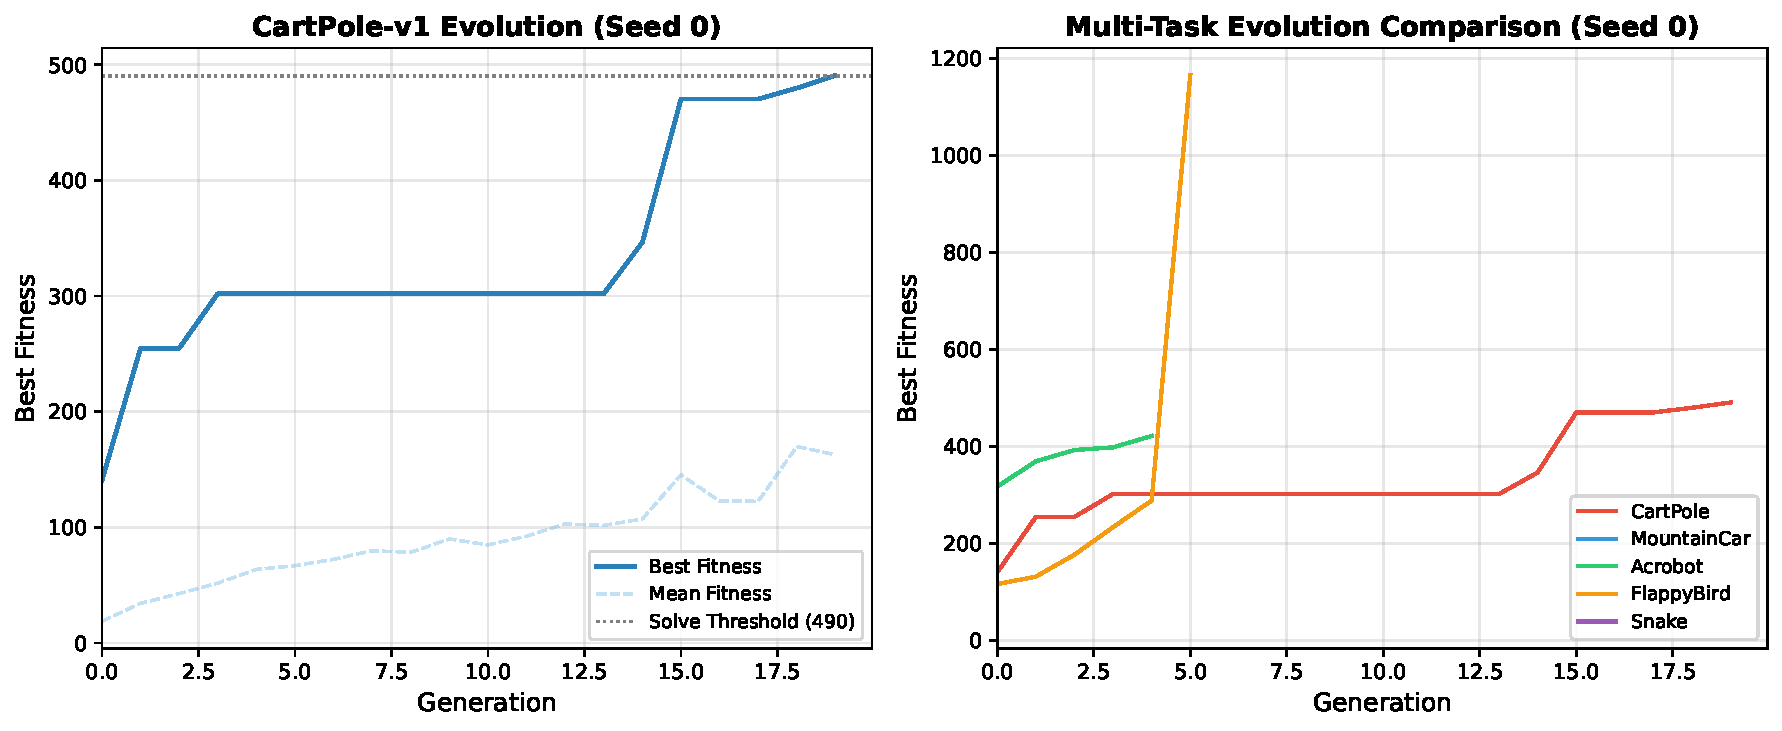
\includegraphics[width=\textwidth]{figures_arxiv/fig01_evolution_curve.pdf}
\caption{\textbf{Evolution curve.} (a)~CartPole-v1 evolutionary trajectory (seed~0): best fitness (solid) and population mean (dashed) over generations, with the CartPole proficiency criterion (490) marked as a dotted line. (b)~Multi-task evolution comparison (seed~0): best-fitness trajectories for CartPole, MountainCar, Acrobot, FlappyBird, and Snake under task-specific shaped fitness functions. All trajectories shown are early-stopped runs within the shared maximum GA budget.}
\label{fig:evolution}
\end{figure}

\subsection{Comparison with weight evolution, NEAT, and PPO}
\label{sec:exp-weight}

The CartPole numbers in this section come from three separate audits: the
multi-task existence run reports task-specific evolutionary and strict-evaluation
scores (Table~\ref{tab:multitask}); the TO/TG/TI experiment is an aligned
co-evolution control whose primary endpoint is the final best-fitness audit
under the aligned evolutionary protocol; and the NEAT/PPO comparison is an
external positioning audit that reuses the 20-seed topology-only CartPole run
where noted. Strict 20-episode re-evaluation values for the CartPole TO/TG/TI
control are included in the released seed-level artifact to make the endpoint
boundary explicit. CartPole is close to the 500-step ceiling, so it is not a
strong benchmark for unrestricted equivalence. Within that ceiling-bound
protocol, however, topology-only evolution (TO) reaches the same performance
regime as co-evolving the global scale (TG) or independent per-synapse weights
(TI, ${\sim}10^4$ continuous parameters): $498.1\pm3.0$ (TO) versus
$497.8\pm3.5$ (TI), with no detectable difference among the three conditions
(one-way ANOVA $F(2,27)=0.44$, $p=0.65$). Under this aligned protocol, removing
per-synapse weight freedom therefore did not produce a detectable CartPole
performance loss, while reducing the continuous synaptic-weight degrees of
freedom by four orders of magnitude. Pairwise mean-difference intervals were
narrow on CartPole: TO--TI was $0.25$ steps (95\% CI $[-2.80,3.30]$), TO--TG
was $1.33$ (95\% CI $[-1.76,4.41]$), and TG--TI was $-1.08$ (95\% CI
$[-4.39,2.24]$). A TOST sensitivity audit makes the margin dependence explicit:
TO--TI is not equivalent under a very tight $\delta=2$ step margin
($p_\mathrm{TOST}=0.12$), but is within a $\delta=5$ step margin
($p_\mathrm{TOST}=0.002$); the minimum symmetric margin supported at
$\alpha=0.05$ is $2.76$ steps. Thus the supported statement is
``no detectable disadvantage, and non-inferiority only under stated margins,''
not unrestricted equivalence.

On MountainCar, with $n=20$ seeds per condition, the sample means rank TG above
TI and TO, but the difference is not statistically resolved. Strict
20-episode fitness is $895.5\pm527.1$ (TO),
$1049.4\pm588.4$ (TG), and $984.0\pm598.9$ (TI), with seed-level success in
$16/20$, $17/20$, and $16/20$ seeds and goal-episode rates of $17.0\%$, $17.8\%$,
and $15.5\%$ respectively. The three groups show no detectable difference under a
one-way ANOVA ($F(2,57)=0.36$, $p=0.70$), a variance-tolerant Welch ANOVA
($F(2,37.9)=0.38$, $p=0.69$), or a non-parametric Kruskal--Wallis test
($H=0.96$, $p=0.62$); Levene's test does not reject variance homogeneity
($p=0.64$), so the unequal-variance concern of smaller samples does not arise
here. The effect size is negligible ($\eta^2=0.013$, $\omega^2\approx0$) and all
three medians sit at $763$--$764$. The top topology-only seed reaches a strict
fitness of $2942.8$, essentially matching the best independent-weight seed
($2945$), indicating that topology-only search does not show a lower observed
upper performance range in this sample and that its mean reflects hit rate rather
than a clear capacity bound. The mean-difference intervals are much wider than
on CartPole: TO--TI was $-88.5$ (95\% CI $[-449.9,272.8]$), TO--TG was
$-153.9$ (95\% CI $[-511.6,203.8]$), and TG--TI was $65.4$ (95\% CI
$[-314.7,445.4]$). Thus the MountainCar result does not rule out modest
advantages or disadvantages of weight freedom; it only shows that no group
effect is statistically resolved in this high-variance setting. The same TOST
sensitivity audit fails at $\delta=300$ shaped-fitness units for TO--TI
($p_\mathrm{TOST}=0.12$) and succeeds only at the broad $\delta=500$ margin
($p_\mathrm{TOST}=0.013$; minimum supported margin $389$). Together with the
CartPole result, this extends the no-detectable-difference finding between
binary topology evolution and weight co-evolution to a second reactive control
task, but with a much wider uncertainty boundary.

As a higher-headroom reactive stress test, we additionally ran the same
TO/TG/TI protocol on discrete LunarLander-v3 ($8$D state, $4$ actions), using a
$128$-neuron controller, $20$ independent seeds per condition, $400$
generations, population $80$, and strict $20$-episode re-evaluation
(Table~\ref{tab:lunarlander-headroom}; Figure~\ref{fig:lunarlander-headroom}).
Before examining this result we specified the primary equivalence margin as
$\delta=0.10|\bar{x}_{\mathrm{TI}}|$, with absolute-margin sensitivity audits at
$25$, $50$, and $75$ reward units. LunarLander provided the intended headroom:
no condition approached the $200$-reward solve threshold. Strict returns were
$-40.0\pm69.9$ for TO, $-82.5\pm37.7$ for TG, and $-53.2\pm41.4$ for TI
(mean $\pm$ seed-level s.d.; $n=20$ each). The ordinary one-way ANOVA detects a
group effect ($F(2,57)=3.55$, $p=0.035$), reflecting that TG is lower in this
sample rather than that independent per-synapse weights outperform topology
only. TO does not show a systematic drop relative to TI: its mean is $13.2$
reward units higher than TI. However, the pre-specified TOST does not support
equivalence under the $10\%$ margin ($\delta=5.32$): for TO--TI the $90\%$ CI is
$[-17.6,44.0]$ and $p_{\mathrm{TOST}}=0.666$. Equivalence is supported only at
broader margins ($\delta=50$ and $75$ reward units; minimum supported symmetric
margin $44.0$). The LunarLander audit therefore removes the CartPole ceiling but
also constrains the central claim: topology-only evolution shows no systematic
disadvantage relative to independent weight co-evolution in this sample, yet
strict small-margin equivalence is not established.

\begin{table}[H]
\centering
\small
\caption{\textbf{LunarLander headroom audit.} Strict 20-episode raw returns for
the aligned TO/TG/TI protocol ($n=20$ seeds per condition). Seed success uses
the conventional LunarLander solve threshold of $200$ reward.}
\label{tab:lunarlander-headroom}
\begin{tabular}{@{}lccc@{}}
\toprule
\textbf{Condition} & \textbf{Strict return} & \textbf{Best seed} & \textbf{Seed success} \\
\midrule
TO & $-40.0\pm69.9$ & $101.1$ & $0/20$ \\
TG & $-82.5\pm37.7$ & $15.6$ & $0/20$ \\
TI & $-53.2\pm41.4$ & $56.1$ & $0/20$ \\
\bottomrule
\end{tabular}
\end{table}

\begin{figure}[H]
\centering
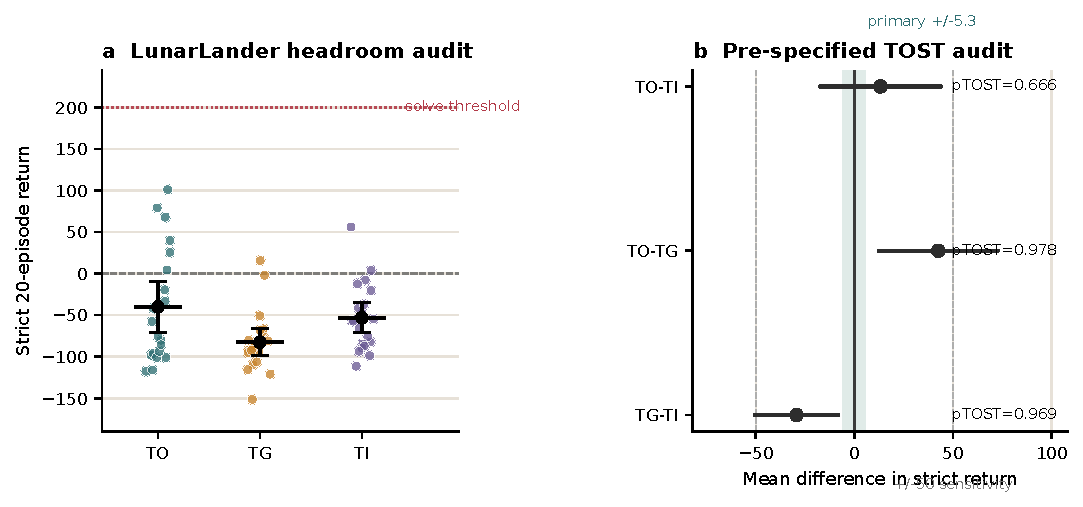
\includegraphics[width=\textwidth]{figures_arxiv/fig15_lunarlander_headroom.pdf}
\caption{\textbf{LunarLander headroom and TOST audit.} (a) Seed-level strict
20-episode raw returns for the aligned TO/TG/TI protocol. Dots are independent
seeds and black bars show mean $\pm$95\% CI. The dashed zero-return line and the
dotted $200$-reward solve threshold show that this audit is not ceiling-bound.
(b) Pairwise mean differences with $90\%$ CIs used for the two-one-sided-tests
audit. The shaded region marks the pre-specified primary margin
($\delta=0.10|\bar{x}_{\mathrm{TI}}|=5.32$ reward units); dashed vertical lines
mark the $\pm50$ reward-unit sensitivity margin.}
\label{fig:lunarlander-headroom}
\end{figure}

For external positioning, rather than as a fairness claim about algorithmic
superiority, we compare the topology-only CartPole audit with NEAT
\citep{stanley2002} and PPO \citep{schulman2017} baselines. NEAT and PPO are run
over $10$ seeds (NEAT: population $50$, recurrent connections allowed; PPO: MLP
$[128,128]$ policy, $200$k timesteps), whereas our method uses the 20-seed
topology-only audit reported above; Table~\ref{tab:comparison} and
Figure~\ref{fig:comparison} summarize the comparison. All three methods reach or
approach the CartPole ceiling: our method $494.7\pm13.8$, NEAT
$494.3\pm12.7$, and PPO $500.0\pm0.0$. The
methods differ in what they expend to get there. PPO uses $34{,}691$
trained parameters and NEAT $11.3\pm1.3$ evolved weights, whereas our controller
has a single global scalar. NEAT converges fastest (median $6$ generations,
${\sim}2{,}400$ evaluations) and, when free to evolve weights, discovers that
CartPole does not require recurrence at all: in $9/10$ seeds it converges to a
$2$--$3$ node, $8$--$11$ connection near-feedforward mapping. Our method instead
holds weights at a single scalar, so solving the same task depends on the
recurrent connection pattern---at the cost of slower convergence (median $85$
generations, ${\sim}34{,}000$ evaluations). The comparison therefore positions
the method in the design space rather than as a faster or stronger controller:
it trades the convergence speed of weight-learning methods for a demonstration
that, on this task, a recurrent connection pattern under a fixed global scale can
reach a comparable performance regime.

\begin{table}[H]
\centering
\footnotesize
\caption{Systematic comparison with NEAT and PPO baselines (CartPole).}
\label{tab:comparison}
\begin{tabularx}{\textwidth}{@{}YYYlYY@{}}
\toprule
\textbf{Method} & \textbf{Final perf.} & \textbf{Median conv.} & \textbf{Continuous params} & \textbf{Network structure} & \textbf{Core mechanism} \\
\midrule
\textbf{Fixed-weight topology evolution (this paper)} & $\mathbf{494.7\pm13.8}$ & 85 gen (${\sim}$34,000 eval) & \textbf{1 scalar} & 128 neurons, recurrent, sparse (${\sim}$41\%) & temporal iterative propagation \\
\textbf{NEAT} & $494.3\pm12.7$ & \textbf{6 gen} (${\sim}$2,400 eval) & $11.3\pm1.3$ & $2.1\pm0.3$ nodes, 8--11 connections & minimal feedforward policy mapping \\
\textbf{PPO} & $500.0\pm0.0$ & ${\sim}$25k timesteps & 34,691 & MLP $[128, 128]$ fixed & gradient-based deep learning \\
\bottomrule
\end{tabularx}
\end{table}

\begin{figure}[htbp]
\centering
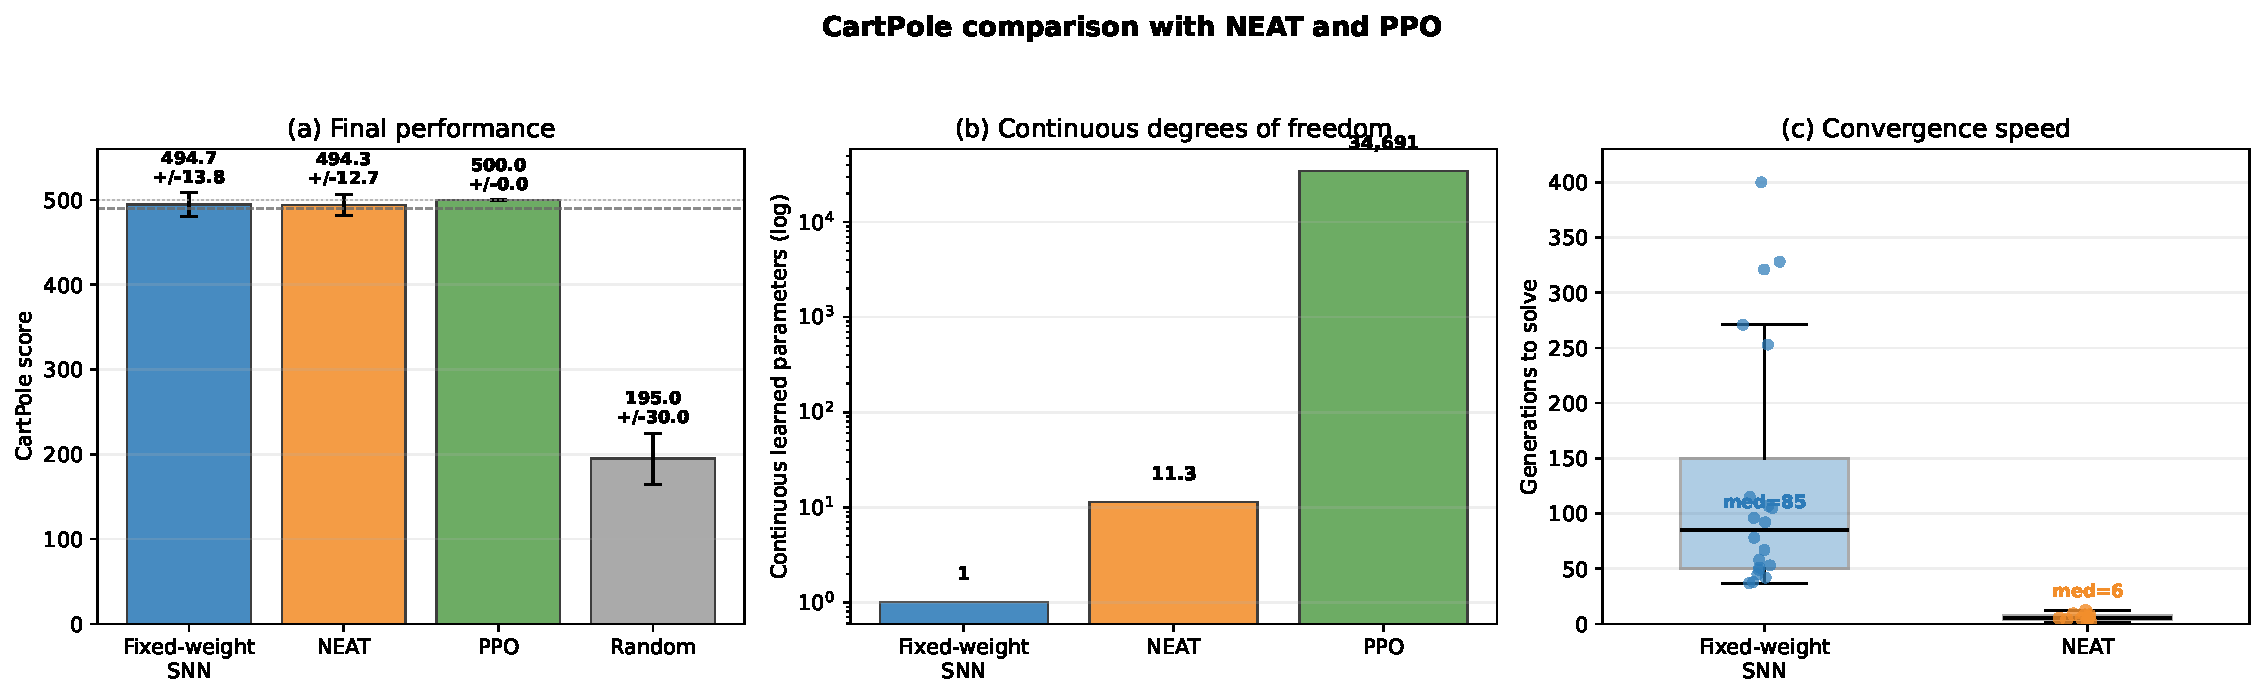
\includegraphics[width=\textwidth]{figures_arxiv/fig12_comparison.pdf}
\caption{\textbf{Systematic comparison with NEAT and PPO baselines (CartPole).} (a) Final performance: fixed-weight topology evolution uses the 20-seed CartPole audit ($494.7\pm13.8$), while NEAT and PPO are 10-seed baselines ($494.3\pm12.7$ and $500.0\pm0.0$); the random reference is approximately $195$. (b) Continuous learned parameter count (log scale): this paper $1$ global scalar, NEAT $\approx 11$, PPO $34{,}691$. (c) Convergence speed (generations to criterion): box plots for the two evolutionary methods, with medians computed from the real seed-level logs.}
\label{fig:comparison}
\end{figure}

\subsection{Temporal iterative propagation as a candidate mechanism}
\label{sec:exp-mechanism}
Several converging analyses indicate that, in our experiments, control
performance depends on the internal rollout length and is consistent with
multi-step temporal propagation through the evolved graph rather than local
connection motifs or precise hidden membrane values alone. The evidence below
should be read as a mechanism audit, not as a complete causal proof: changing
$T_\text{steps}$ also changes the opportunity for output spikes to accumulate,
and the history analyses are observational. Following
Section~\ref{sec:decoding}, the analyses below separate temporal iterative
propagation ($T_\text{steps}$) from structural recurrence (cycles or hidden-layer
recurrent edges).

\paragraph{Temporal iteration is necessary.}
Reducing an evolved topology's internal passes from $T_\text{steps}=20$ to
$T_\text{steps}=1$ (preventing multi-step temporal propagation without deleting
any recurrent edges) sharply reduces performance:
CartPole drops from ${\sim}438$ to ${\sim}9$ ($98\%$), FlappyBird from ${>}100$ to
${\sim}5$ ($95\%$), and MountainCar fails entirely to escape the valley
(Table~\ref{tab:tsteps-ablation}). The continuous $T_\text{steps}$ curve on
CartPole rises from $9$ at $T{=}1$ to $25$ at $T{=}5$, jumps to $380$ at $T{=}10$,
and saturates near $438$ at $T{=}20$ (Figure~\ref{fig:tsteps}), so the evolved
topology actively depends on multi-step temporal iteration.

\paragraph{Precise hidden membrane values alone are not the carrier.}
Resetting hidden-layer membrane potentials to zero at an intermediate step of the
$T_\text{steps}=20$ forward pass does not impair performance (all drops
$<0.5$, within evaluation noise), yet the membrane traces show sustained spiking
rather than relaxation to a fixed state (Figure~\ref{fig:membrane}). This
perturbation does not rule out all state variables, but it argues against the
precise instantaneous hidden membrane vector being the sole carrier of function;
control instead appears to depend on propagation paths---signals
propagating and mixing over multiple steps.

\paragraph{Input history is linearly decodable, with a task-matched window.}
A Ridge decoder trained to predict past inputs from current hidden activity
recovers recent history, and the decodable window matches the task timescale. On
CartPole, decoding rises from $R^2<0$ at $T{=}1$ to $R^2\approx0.56$ at $T{=}3$
and $R^2\approx0.63$ at $T{=}5$ (best dimension, cart velocity, $\approx0.85$),
reaching $R^2\approx0.75$ at $T{=}20$---a rapid rise consistent with reactive
control. On MountainCar, decoding is optimal at $T{=}20$ (position
$R^2\approx0.59$, velocity $R^2\approx0.74$) and decays slowly (at $T{=}20$, a
lag-4 input is still decodable at $R^2\approx0.61$), while at $T{=}30$ it degrades
($R^2\approx0.44$). Reactive tasks thus use short recurrence and integrative tasks
longer recurrence (Figure~\ref{fig:decoding}).

\paragraph{Output spike timing is history-dependent.}
Restricting analysis to steps where the pole is near vertical
($|\text{pole\_angle}|<0.05$) and stratifying by recent velocity history, output
spike timing still differs with recent history. As a descriptive distributional
summary over sampled time steps, both output neurons show shifted first-spike
times between positive- and negative-velocity history conditions. Adjacent time
steps are autocorrelated, so we do not treat time-indexed $t$-tests as
independent-trial inference; the corresponding descriptive values are
push-left $t=53.21$ and push-right $t=-39.15$, with sign set by comparison
order. The more robust readout is the accompanying spike-count shift: the
push-right neuron wins $85.1\%$ of steps under rightward-leaning history versus
$16.0\%$ under leftward-leaning history (Figure~\ref{fig:spike_timing}). Because
matching only the pole angle does not fully match cart position, cart velocity,
and pole angular velocity, we treat this panel as descriptive evidence for a
history-conditioned readout rather than definitive proof that all current-state
confounds have been eliminated.

\paragraph{A rate-substitution control does not recover the policy.}
Because the discrete-action readout uses accumulated output spike counts, a
natural alternative explanation is that the controller is merely an iterated
non-spiking rate map. We therefore replaced threshold-and-reset spiking on the
same evolved CartPole topology with continuous sigmoid, tanh, or clipped-ReLU
rate nonlinearities over a gain grid, leaving the topology, Dale signs, global
scale, and $T_\text{steps}$ unchanged. This substitution is intentionally a
mechanistic control rather than a freshly evolved rate-network baseline. The
spiking LIF controller scored $460.2\pm61.6$ over the matched 20-episode
evaluation, whereas the best rate-substitution variant reached only
$12.2\pm1.4$ steps (clipped-ReLU, gain $0.5$). The result does not prove that no
rate network could solve the task after re-evolution, but it shows that the
evolved fixed-weight policy is not reproduced by simply replacing spikes with a
smooth iterated rate update.

\begin{table}[H]
\centering
\caption{$T_\text{steps}$ ablation results.}
\label{tab:tsteps-ablation}
\begin{tabular}{@{}lccc@{}}
\toprule
\textbf{Task} & \textbf{$T=20$ (baseline)} & \textbf{$T=1$} & \textbf{Drop} \\
\midrule
CartPole & ${\sim}438$ & ${\sim}9$ & 98\% \\
MountainCar & 0.28 & $-$0.50 & 100\%$^*$ \\
FlappyBird & ${>}100$ & ${\sim}5$ & 95\% \\
\bottomrule
\end{tabular}
\end{table}

\noindent$^*$MountainCar is evaluated by maximum position (goal${=}0.5$); $T{=}1$ cannot escape the valley.

\begin{figure}[htbp]
\centering
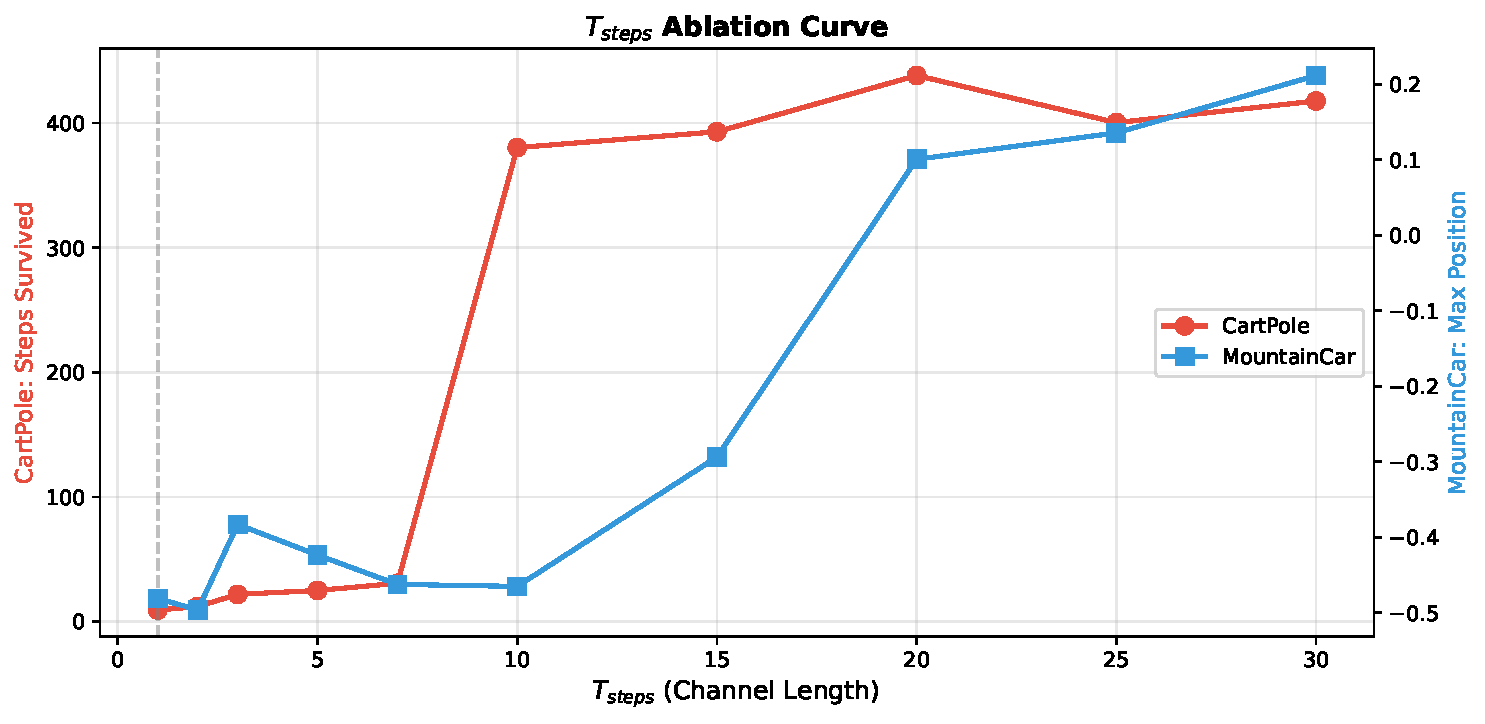
\includegraphics[width=\textwidth]{figures_arxiv/fig02_tsteps_curve.pdf}
\caption{\textbf{$T_\text{steps}$ ablation curve (CartPole).} Performance of the evolved CartPole topology evaluated at different $T_\text{steps}$ values: $T=1$ gives 9 (no multi-step temporal iterative propagation), $T=5$ gives 25, $T=10$ jumps to 380, $T=15$ reaches 393, $T=20$ saturates at 438, $T=25$ at 400. The 10-episode mean is shown with $\pm$std shading.}
\label{fig:tsteps}
\end{figure}

\begin{figure}[htbp]
\centering
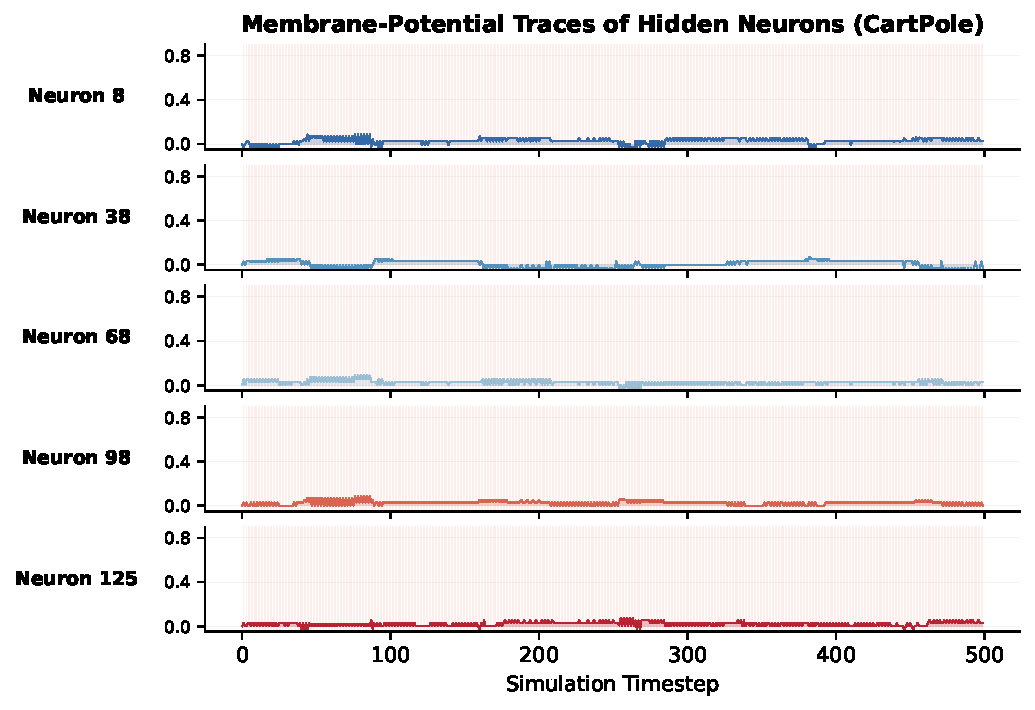
\includegraphics[width=\textwidth]{figures_arxiv/fig03_membrane_traces.pdf}
\caption{\textbf{Membrane-potential trajectories (CartPole).} Membrane potential of five representative hidden neurons (N8, N38, N68, N98, N125) over the first 500 simulation timesteps. The traces reveal sustained spiking activity rather than a stable equilibrium, consistent with the interpretation that information is carried in the ongoing propagation of signals rather than in precise hidden membrane values alone.}
\label{fig:membrane}
\end{figure}

\begin{figure}[htbp]
\centering
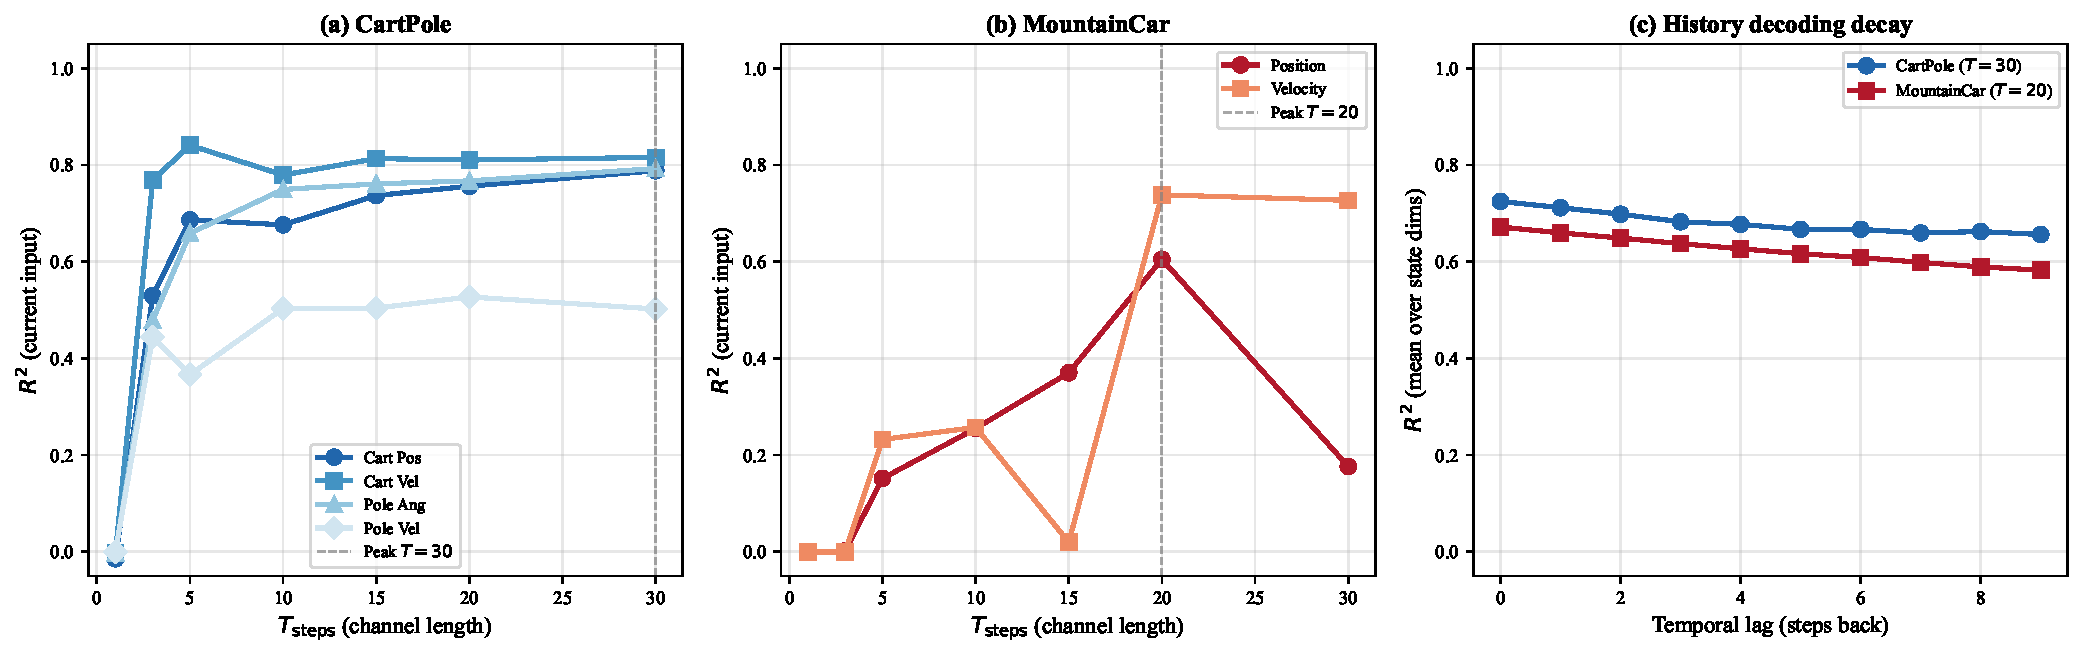
\includegraphics[width=\textwidth]{figures_arxiv/fig04_input_decoding.pdf}
\caption{\textbf{Decoding input history from hidden activity.} (a) CartPole: $R^2$ of decoding each of the 4 state dimensions from the hidden-layer spike-count accumulation at different $T_\text{steps}$ values, rising sharply at $T{=}3$--$5$ (best dimension Cart Vel $\approx 0.85$ at $T{=}5$). (b) MountainCar: $R^2$ of decoding the 2 state dimensions (position, velocity), peaking at $T{=}20$ (velocity $\approx 0.74$, position $\approx 0.59$). (c) History decay: at the optimal $T$ for each task, $R^2$ as a function of how many steps back the queried input lies. MountainCar retains a strong decodable signal even at lag${=}4$ ($R^2{\approx}0.61$), while CartPole decays more rapidly.}
\label{fig:decoding}
\end{figure}

\begin{figure}[htbp]
\centering
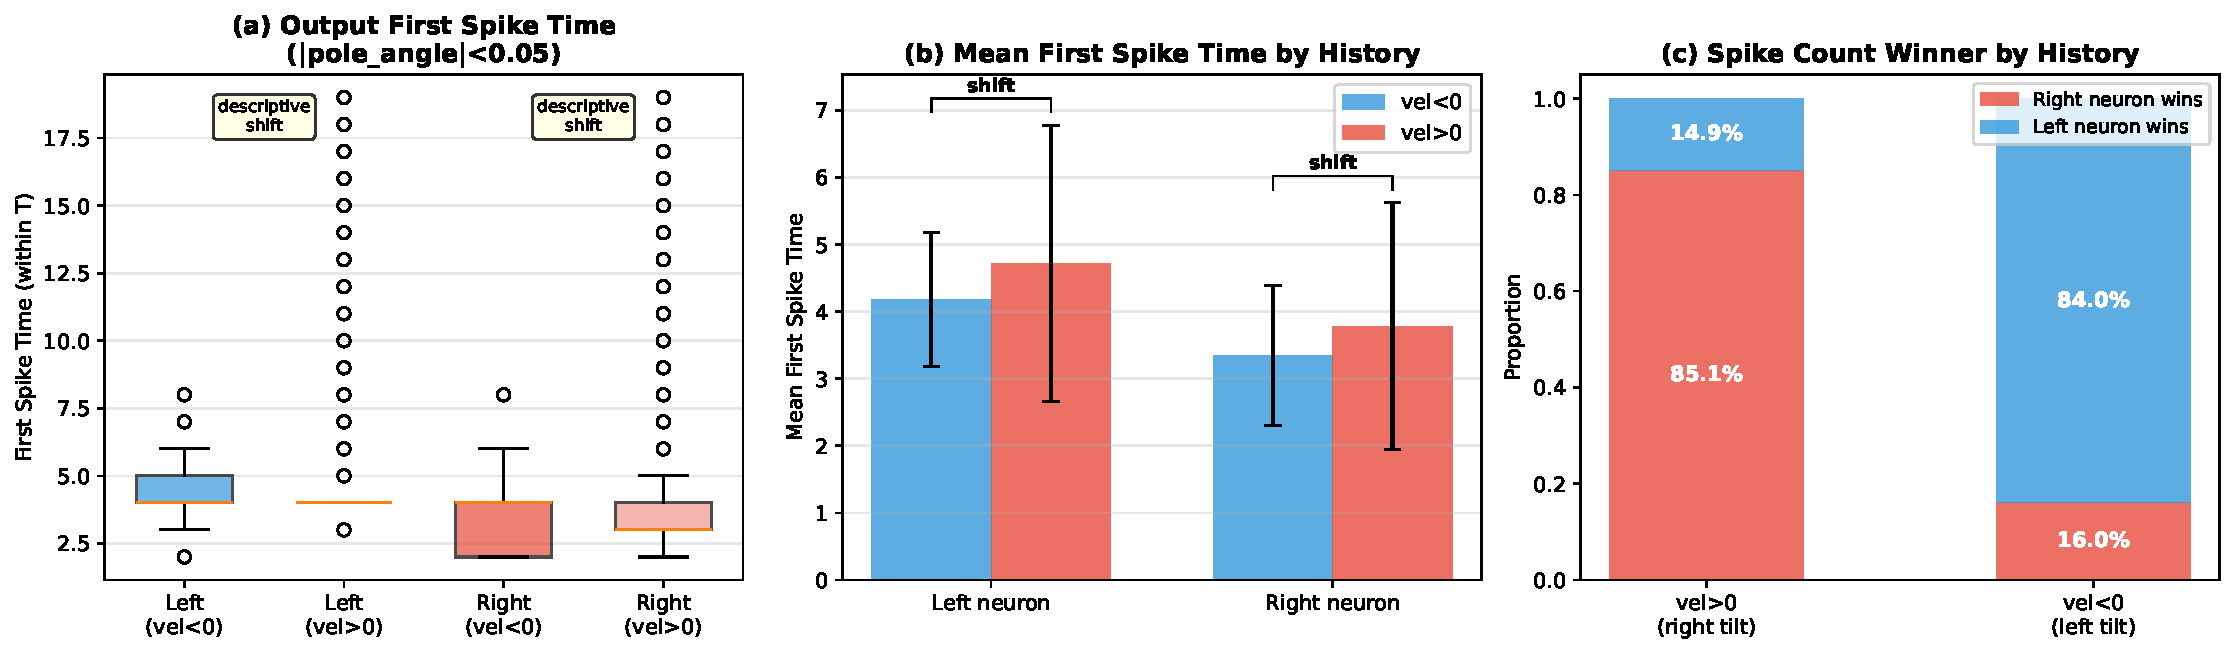
\includegraphics[width=\textwidth]{figures_arxiv/fig06_spike_timing.pdf}
\caption{\textbf{Modulation of output spike timing by history.} (a) Box plot of the first-spike time of the push-left and push-right output neurons under the two history conditions, with the current input held nearly constant ($|\text{pole\_angle}|<0.05$); two-sample $t$-tests over sampled time steps are shown as descriptive distributional summaries because adjacent steps are autocorrelated. (b) Mean first-spike time by history condition; markers denote descriptive distributional shifts, not independent-trial inference. (c) Spike-count winner by velocity sign: under rightward-leaning history (vel${>}0$), the right neuron wins 85.1\% of steps; under leftward-leaning history (vel${<}0$), the right neuron wins only 16.0\% of steps and the left neuron wins 84.0\%.}
\label{fig:spike_timing}
\end{figure}

\subsection{Connection-type ablation and motif analysis}
\label{sec:exp-ablation}

We probe whether function resides in specific local connection patterns (network
motifs; \citealp{milo2002}). For 2-node E/I connection classes, motif $z$-scores against degree-matched random
networks are all $|z|<2.0$ (no enrichment); among 512 3-node patterns, only
CartPole shows weak enrichment ($43/512$ with $|z|>2$, concentrated in dense
E-E-E clusters) and Snake shows none. These analyses therefore provide little
support for a mechanism dominated by repeated local circuits. A systematic connection-type ablation
(Table~\ref{tab:ablation}) shows that robustness depends mainly on the number of
connections rather than their E/I arrangement: deleting E$\rightarrow$E (53\% of
edges) is the most destructive in absolute terms ($415.4\to9.3$ steps) but its
specificity index ($+0.12$) is uninterpretable at that ablation scale, while the
I$\rightarrow$E and E$\rightarrow$I specificity indices are negative
($-0.20$, $-0.21$). Layered ablation confirms that the feedforward through-path
can suffice for the basic CartPole mapping once multiple temporal passes are
retained (disconnecting the hidden layer internally: $427.5$; disconnecting the
input layer: $78.8$; Figure~\ref{fig:ablation}). Thus the necessary component in
Section~\ref{sec:exp-mechanism} is temporal iterative propagation, not an
unqualified requirement for hidden-layer cycles on every solved task.

\begin{table}[H]
\centering
\footnotesize
\caption{Systematic connection-type ablation results ($\mathit{weight\_scale}=0.6$, consistent with the evolution configuration). Baseline performance $415.4 \pm 18.6$ steps (mean of 20 episodes, 5 evaluations).}
\label{tab:ablation}
\begin{tabularx}{\textwidth}{@{}lYYYYY@{}}
\toprule
\textbf{Ablation condition} & \textbf{Edges deleted} & \textbf{Post-ablation perf.} & \textbf{Random-control perf.} & \textbf{Specificity index} & \textbf{Functional reading} \\
\midrule
\textbf{Delete E$\rightarrow$E} & 3,569 (53\%) & \textbf{9.3} & ${\sim}328$ & $+$0.12 & share too large; index uninterpretable \\
Delete I$\rightarrow$E & 1,303 (19\%) & 125.2 & ${\sim}314$ & $-$0.20 & arrangement not specific \\
Delete E$\rightarrow$I & 1,329 (20\%) & 137.9 & ${\sim}303$ & $-$0.21 & arrangement not specific \\
\textbf{Delete I$\rightarrow$I} & 484 (7\%) & \textbf{47.4} & ${\sim}259$ & undecidable ($+$0.27) & variance too large; undecidable \\
\bottomrule
\end{tabularx}
\end{table}

\begin{figure}[htbp]
\centering
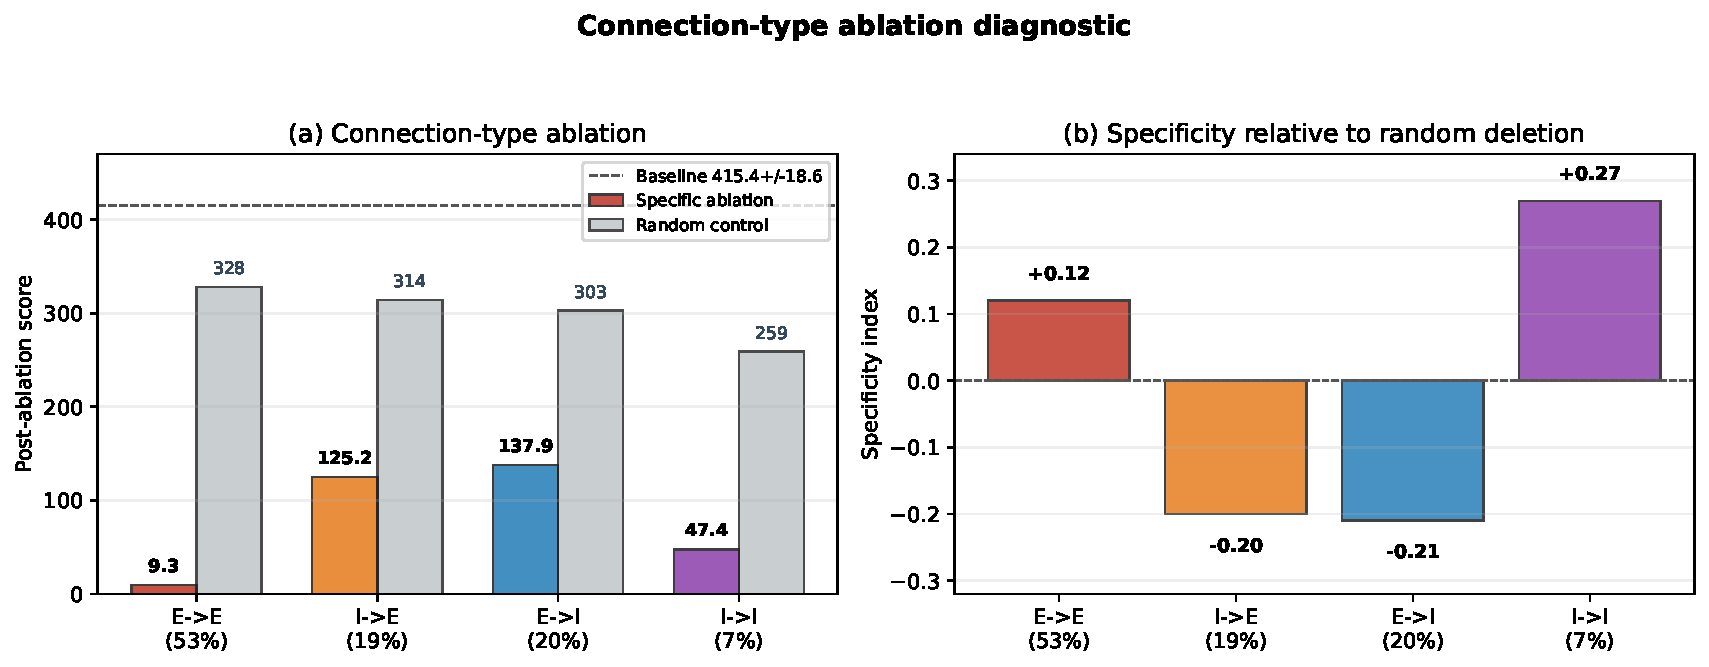
\includegraphics[width=\textwidth]{figures_arxiv/fig07_connection_ablation.pdf}
\caption{\textbf{Systematic connection-type ablation.} Comparison of the performance drop of specific ablation (red) and random-control ablation (blue, mean$\pm$std) ($\mathit{weight\_scale}=0.6$). Note that E$\rightarrow$E accounts for 53\% of all connections, and both specific and random ablation cause near-complete performance collapse, so the specificity index ($+$0.12) lacks discriminative power. I$\rightarrow$I accounts for only 7\%, but the variance of its random control is extremely large ($\pm72.0$, coefficient of variation 28\%), so the apparent specificity index ($+$0.27) is marked undecidable rather than interpreted.}
\label{fig:ablation}
\end{figure}

\subsection{Task/configuration-specific structural fingerprints}
\label{sec:exp-fingerprint}

Across the five discrete task configurations, $50$ independently evolved
topologies ($10$ per task) form configuration-separable structural fingerprints
(Figure~\ref{fig:fingerprint}). A leave-one-out KNN classifier assigns source
configuration at $94.0\%$ accuracy (versus $20\%$ chance), with E/I ratio, path
length, and degree entropy the most discriminative structural features. The only
misclassifications occur between FlappyBird and MountainCar, two low-dimensional
tasks ($8/10$ and $9/10$ correct, respectively). A Mantel test between structural
distance and hand-crafted task-metadata distance is not significant
($r=0.433$, exact label-permutation $p=0.308$); with only five task-level points,
this test has low power and should not be read as strong evidence for the
absence of a task--structure relationship.

We therefore audit the architecture confound directly. The five tasks differ in
network size and input/output interface, and those metadata alone
($N,n_\text{in},n_\text{out}$) classify the task labels perfectly in this data
set. After linearly residualizing the 19 structural features against these
architecture metadata, LOO-KNN accuracy drops from $94.0\%$ to $48.0\%$; using a
larger metadata set that also includes state and action dimension gives the same
$48.0\%$. Conversely, within the fixed-$N=128$ subset (CartPole versus Acrobot),
structural features still separate the two tasks at $100\%$ accuracy, although
this subset remains confounded by I/O dimensionality and contains only two
tasks. We therefore claim only that the evolved graphs carry
configuration-identifiable structure. The analysis does not establish an
architecture-independent task fingerprint.

\begin{figure}[htbp]
\centering
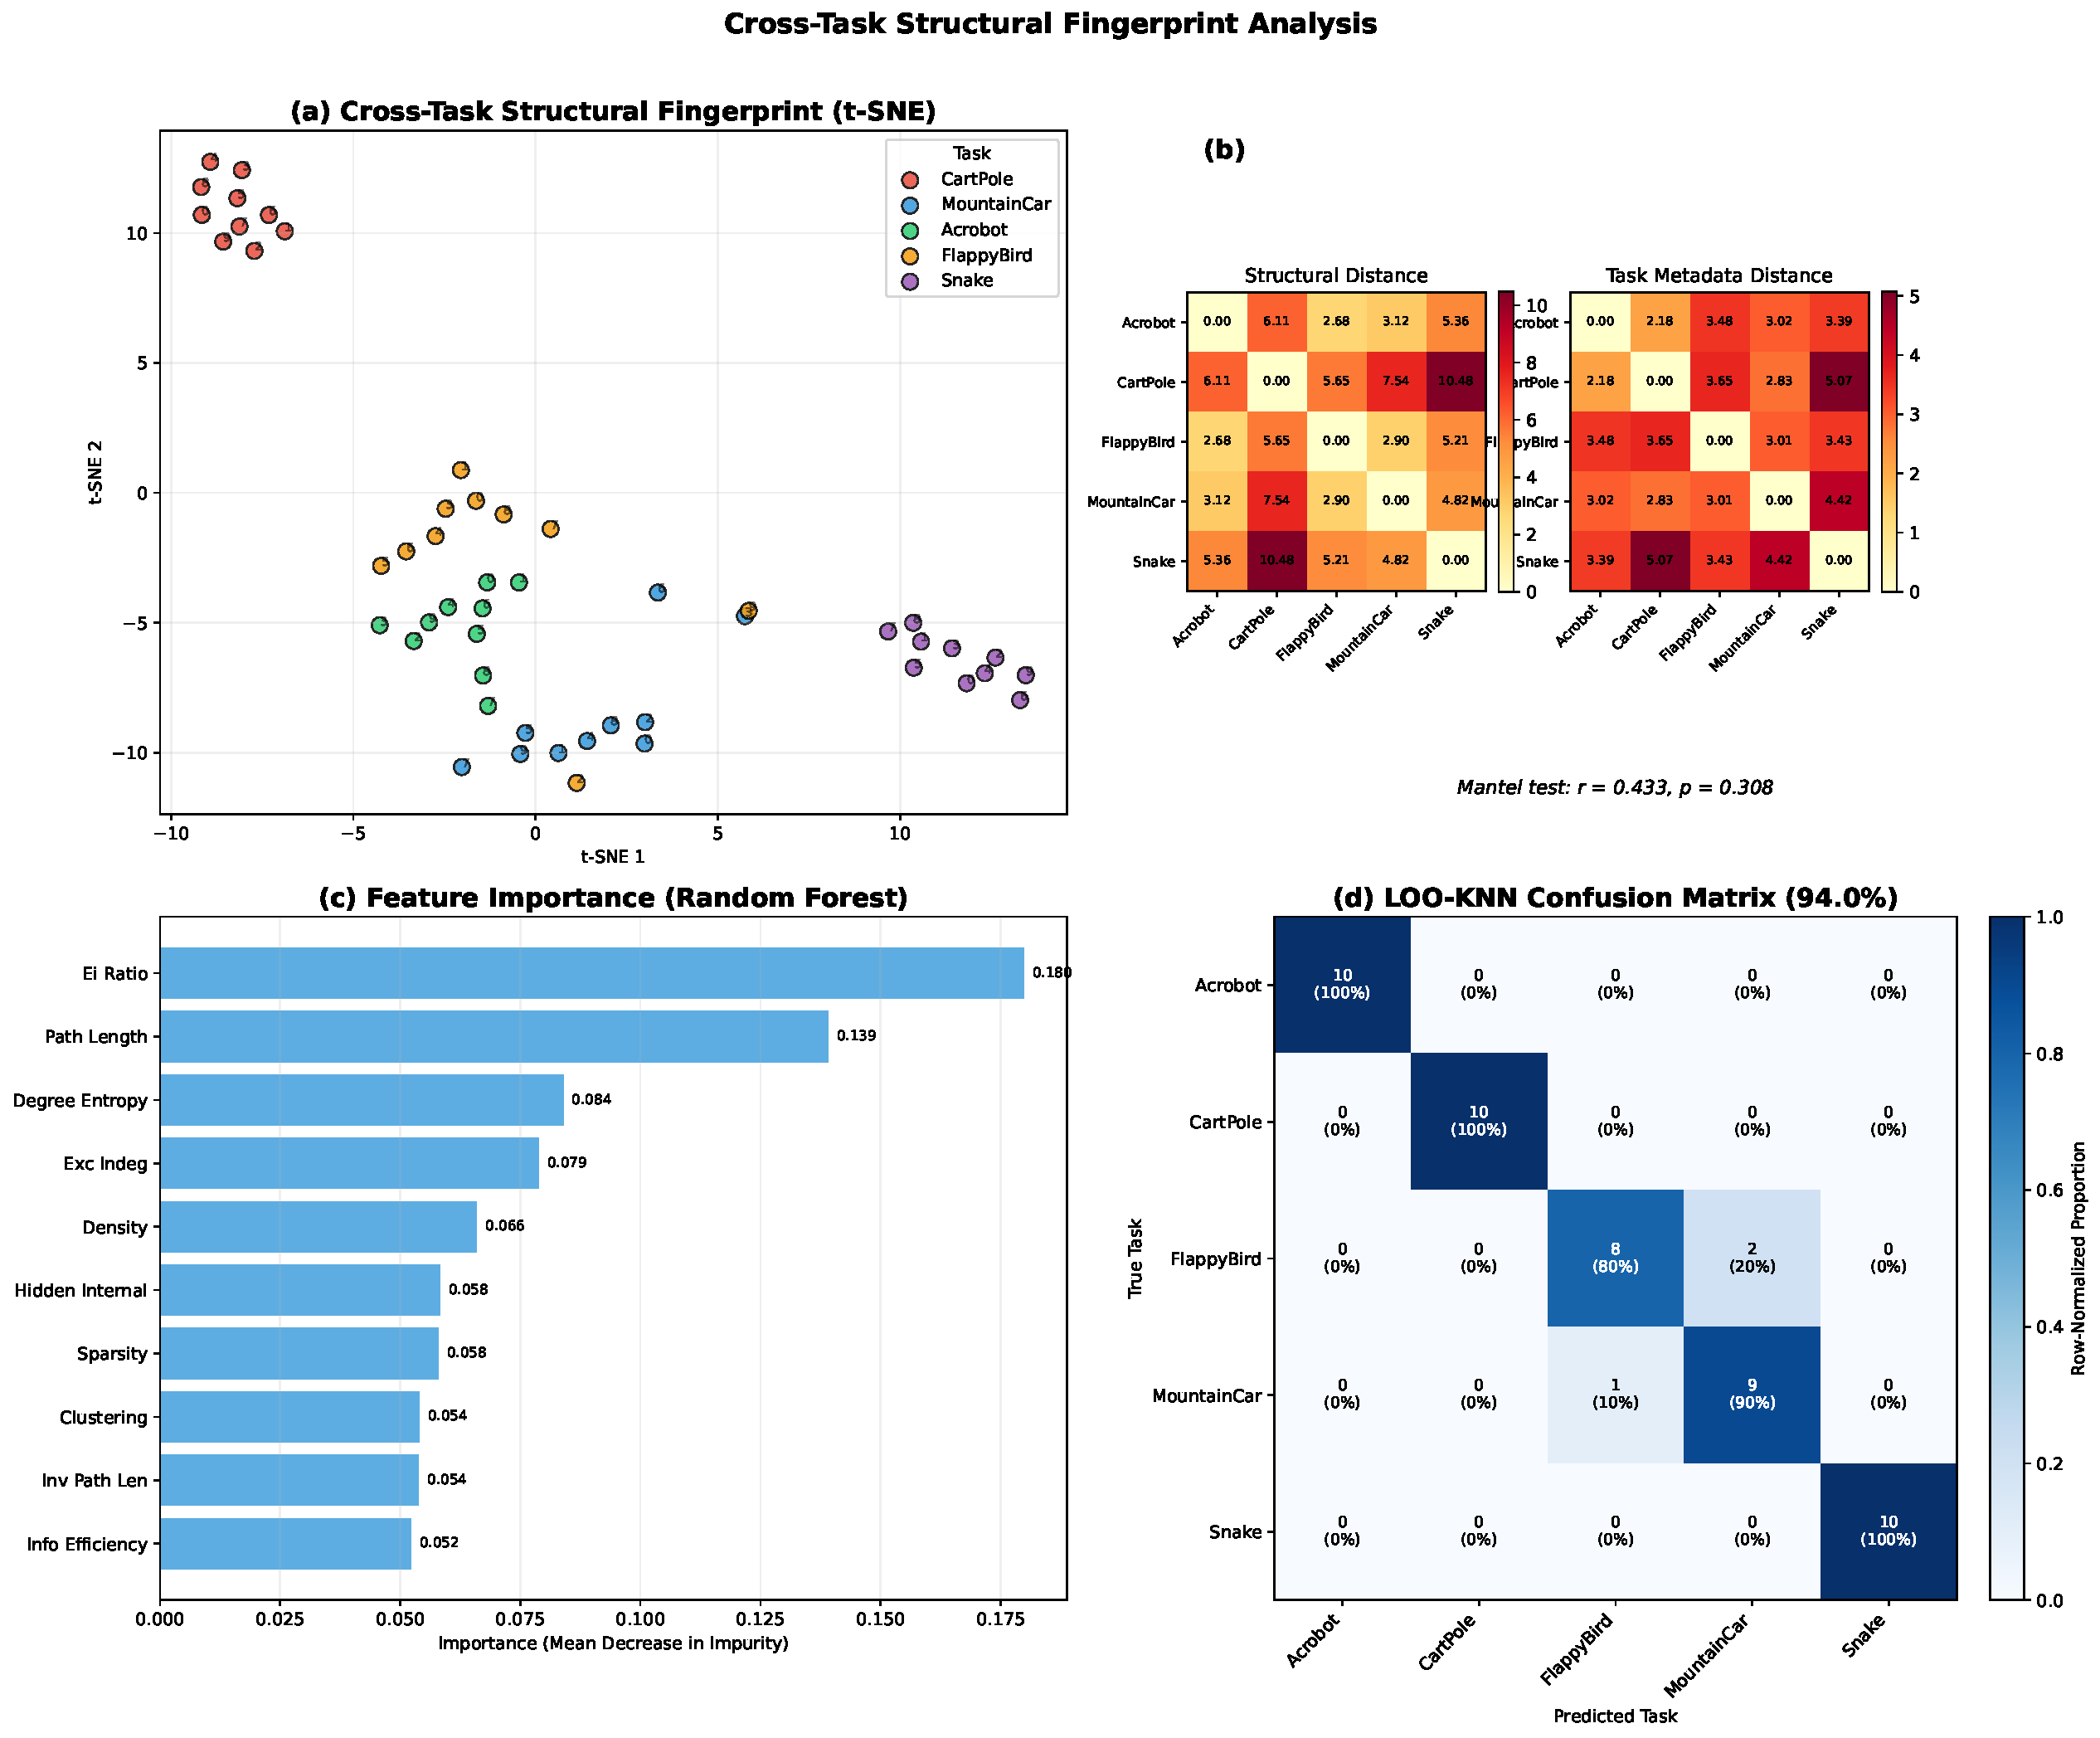
\includegraphics[width=\textwidth]{figures_arxiv/fig13_fingerprint.pdf}
\caption{\textbf{Cross-task structural fingerprints.} Fifty topologies (10 per task) evolved on the five discrete task configurations, characterized by 19 structural features. Because task identity is coupled to task-specific network size and input/output dimensions, the analysis identifies configuration-separable structural signatures rather than an architecture-independent task metric. (a) t-SNE projection of the structural features, colored by task. (b) Structural-distance and task-metadata-distance matrices used for the Mantel test ($r=0.433$, exact label-permutation $p=0.308$; low powered because $n=5$ task-level points). (c) Random-forest feature importance; the most discriminative features are E/I ratio, path length, and degree entropy. (d) Leave-one-out KNN confusion matrix (overall accuracy $94.0\%$); the only confusions are between FlappyBird and MountainCar. A metadata audit shows that architecture metadata alone also classify task labels in this data set, and residualizing structural features against $N,n_\text{in},n_\text{out}$ lowers accuracy to $48.0\%$.}
\label{fig:fingerprint}
\end{figure}

\subsection{Continuous-control extension}
\label{sec:exp-continuous}

The continuous-control experiments test whether the same fixed-weight
topology-only design can be evaluated beyond discrete action selection. On
Pendulum-v1, the controller improves over a random policy, reaching $-761.6$
under strict 20-episode evaluation ($43.0\%$ above random) and a best evolved
score of $-678.2$ ($49.3\%$ above random), against a random
baseline of $-1336.6$ (Figure~\ref{fig:embodied}d). On Hopper-v4, a $64$-neuron
controller with a single global weight-scale parameter reaches $1009.1\pm2.8$
under strict 20-episode evaluation (Figure~\ref{fig:embodied}a,b), rising during
evolution from $99$ to $643$ to $987$ over generations 6--8 and plateauing near
$1009$ by generation 53. This corresponds to $48.4\%$ of a 1M-step PPO reference
averaged over three seeds ($2083.7$ mean reward; $36{,}615$ parameters, i.e.\
$36{,}615$-fold more continuous parameters than the SNN). Because the PPO
reference itself shows high seed-to-seed variance (1M-step per-seed returns
$1376$, $1339$, and $3535$), we use this comparison as a scale reference rather
than a claim of PPO-level locomotion. This single-topology result suggests that
fixed per-synapse weights need not restrict the design to discrete control:
recurrent topology can support a low-dimensional continuous-locomotion
proof-of-concept. Moreover, after retuning only the global weight scale (from
$0.5$ to $0.6$), the same evolved topology retains $980.8$ and $982.0$ reward
under $1.3\times$ and $1.5\times$ gravity (Figure~\ref{fig:embodied}c), about
$97\%$ of its standard-gravity score ($1014.4$), indicating that adaptation to a
changed environment can, in this instance, proceed by tuning a single scalar
rather than re-evolving the topology. We note that the continuous-control results come from a single evolved
topology (seed~42) evaluated over episodes: the Hopper $\pm2.8$ is episode-level
rather than seed-level variability, and the Pendulum values are a strict
20-episode mean plus a best evolutionary score rather than seed-level statistics.
We therefore treat the continuous-control extension as a proof-of-concept rather
than a multi-seed benchmark, in contrast to the discrete tasks evaluated over
10--20 seeds. At the
same time, the remaining gap to PPO, the absence of seed-level replication, and
the failures on higher-dimensional action spaces (Section~\ref{sec:exp-boundary})
indicate a clear boundary of the present one-scale, 64--128 neuron architecture.

\begin{figure}[htbp]
\centering
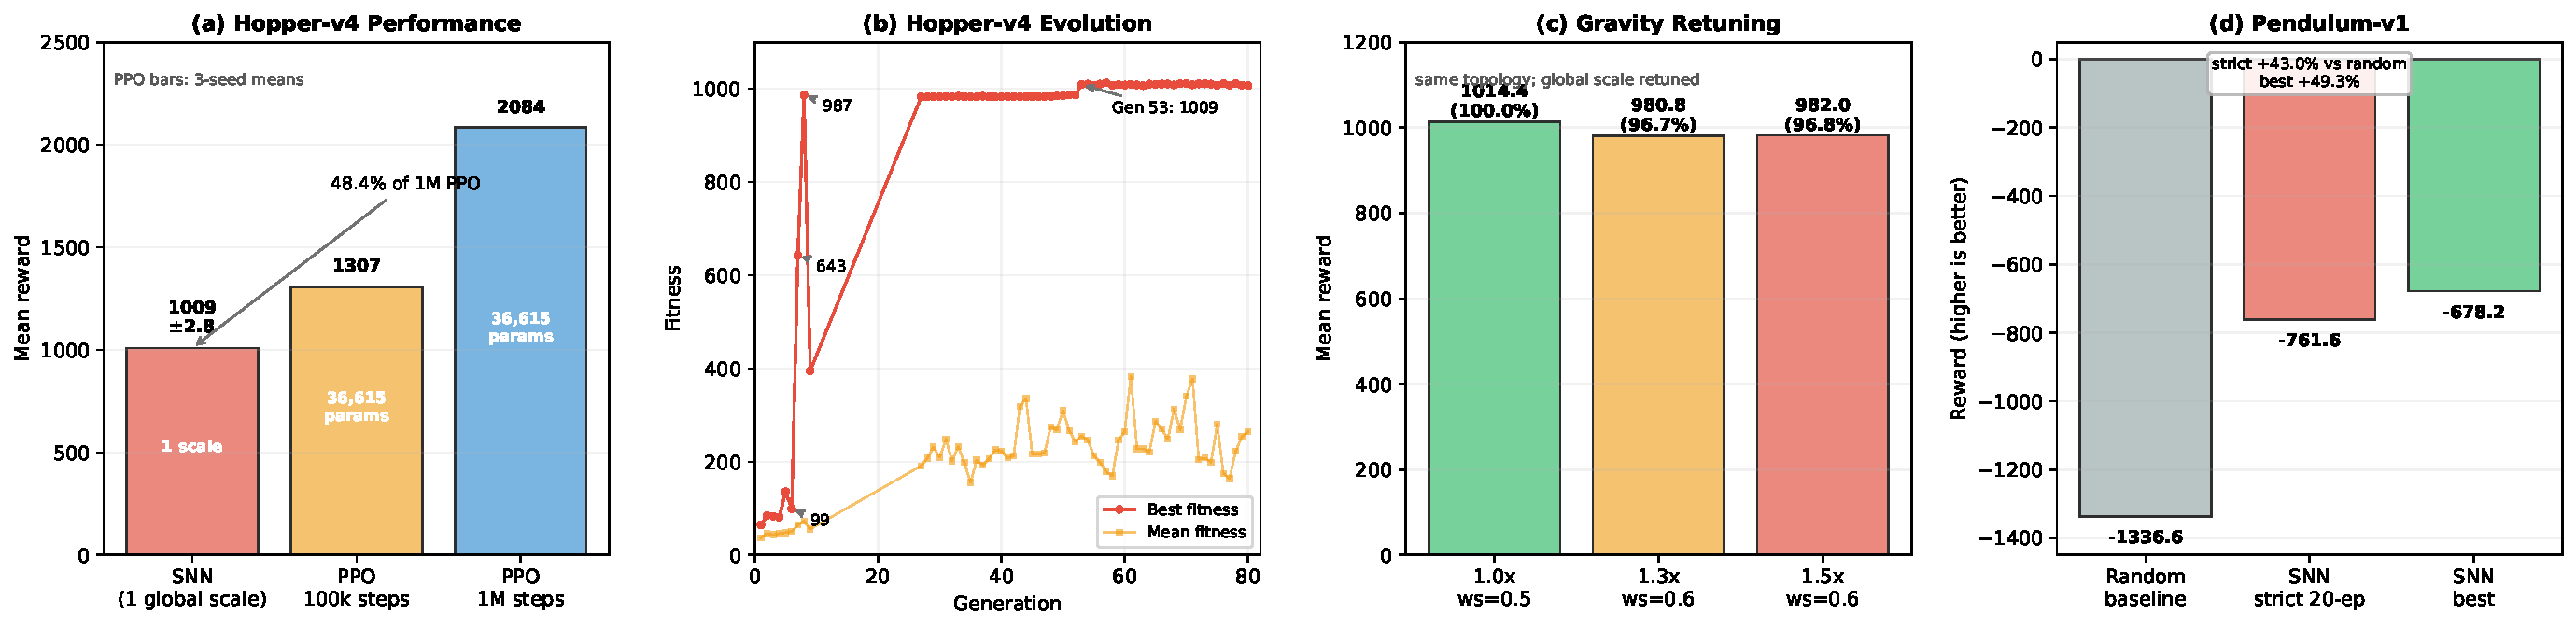
\includegraphics[width=\textwidth]{figures_arxiv/fig14_embodied_control.pdf}
\caption{\textbf{Continuous-control extension.} (a) Hopper-v4 performance. A 64-neuron fixed-weight SNN reaches $1009.1\pm2.8$ under strict 20-episode evaluation with a single global weight-scale parameter. This is a single evolved topology (seed 42), and the $\pm2.8$ interval is episode-level rather than seed-level variability. For scale, PPO references trained for 100k and 1M steps reach $1307.2$ and $2083.7$ mean reward across three seeds (36,615 parameters). (b) Hopper-v4 evolution. Fitness rises sharply from 99.3 to 643.0 to 986.8 over generations 6--8, then stays near 983--1013, with a later increase to 1008.9 at generation 53. (c) Gravity perturbation after global-scale retuning. The same topology reaches 1014.4 at standard gravity (scale 0.5) and retains 980.8--982.0 reward under $1.3\times$ and $1.5\times$ gravity (scale 0.6), about 97\% of the standard-gravity score. (d) Pendulum-v1 proof-of-concept. The SNN improves over the random baseline ($-1336.6$), reaching $-761.6$ under strict 20-episode evaluation ($43.0\%$ above random) and a best evolved score of $-678.2$ ($49.3\%$ above random).}
\label{fig:embodied}
\end{figure}

\subsection{Boundary conditions and adaptation}
\label{sec:exp-boundary}

\paragraph{Working memory.}
On the fixed-delay working-memory tasks (Ghost Hunter and Direction Hold), which
require storing a discrete bit across a blank interval, the fixed-weight
controller remained near chance, with accuracies of $23$--$54\%$. These failures
are consistent with the LIF dynamics: with $20\%$ leakage per propagation step
and no learnable recurrent weights, the network does not form stable
attractor-like states for retaining a discrete bit across a delay. This delimits
reactive control and short-timescale integration, which the method supports, from
discrete working memory, which it does not.

\paragraph{Zero-shot cross-task transfer.}
A topology evolved on one task configuration does not transfer zero-shot to
another under the embedding protocol described in Section~\ref{sec:protocol}:
direct transfer (for example, FlappyBird to MountainCar) yields random-level
performance, and mean off-diagonal transfer is $0.12$ of native performance
(best $0.31$; Figure~\ref{fig:cross_task}). Together with the fingerprint result
(Section~\ref{sec:exp-fingerprint}), this indicates that the evolved recurrent
paths are specialized to the task on which they were selected: task identity is
decodable from structure, yet that structure is not a reusable general
controller.

\paragraph{Action-dimensionality boundary.}
At the present network scale ($64$--$128$ neurons), the method does not reach
proficiency on higher-dimensional action spaces. On HalfCheetah-v4 (6D action
space), the original topology-only protocol reaches only $-415.5$, below the
pre-specified boundary threshold of $-200$. We also tried three escape
strategies---quality-diversity search, larger populations, and per-output
independent weights---which improved the score to $-260.5$, $-227.4$, and
$-241.3$, respectively, but none crossed this boundary. Thus the best observed
HalfCheetah score in this set of boundary tests is $-227.4$. This
suggests that the failure is not due to a single unlucky search setting, but we
report it as a current boundary rather than a proven architectural limit, since
search, readout, and network scale are not separately ruled out.

\paragraph{Low-dimensional adaptation under abrupt change.}
Finally, we tested low-dimensional post-hoc adaptation under environmental
change (Figure~\ref{fig:adaptation}). On CartPole, increasing gravity from $9.8$
to $15.0$ produces a direct stress test of performance retention. The fixed
topology did not collapse: zero-shot performance was $375$ steps against a
standard-gravity baseline of $500$. Retuning only the global weight scale
improved performance to $424$ steps, and retuning only $T_\text{steps}$ reached
$394$. We report absolute scores rather than treating these as formal recovery
percentages, since the achievable ceiling itself shifts under changed gravity
and the pre- and post-change scores are not strictly comparable. We read this not
as a fair competition with PPO but as evidence that a fixed topology offers a
low-dimensional adaptation path---a single global scalar or an internal
iteration depth---under abrupt environmental shift. The source data,
Figure~\ref{fig:adaptation}, and caption use the same four summary values
($500$, $375$, $424$, and $394$); these are absolute 20-episode means, not
renumbered figure indices or recovery percentages.

\begin{figure}[htbp]
\centering
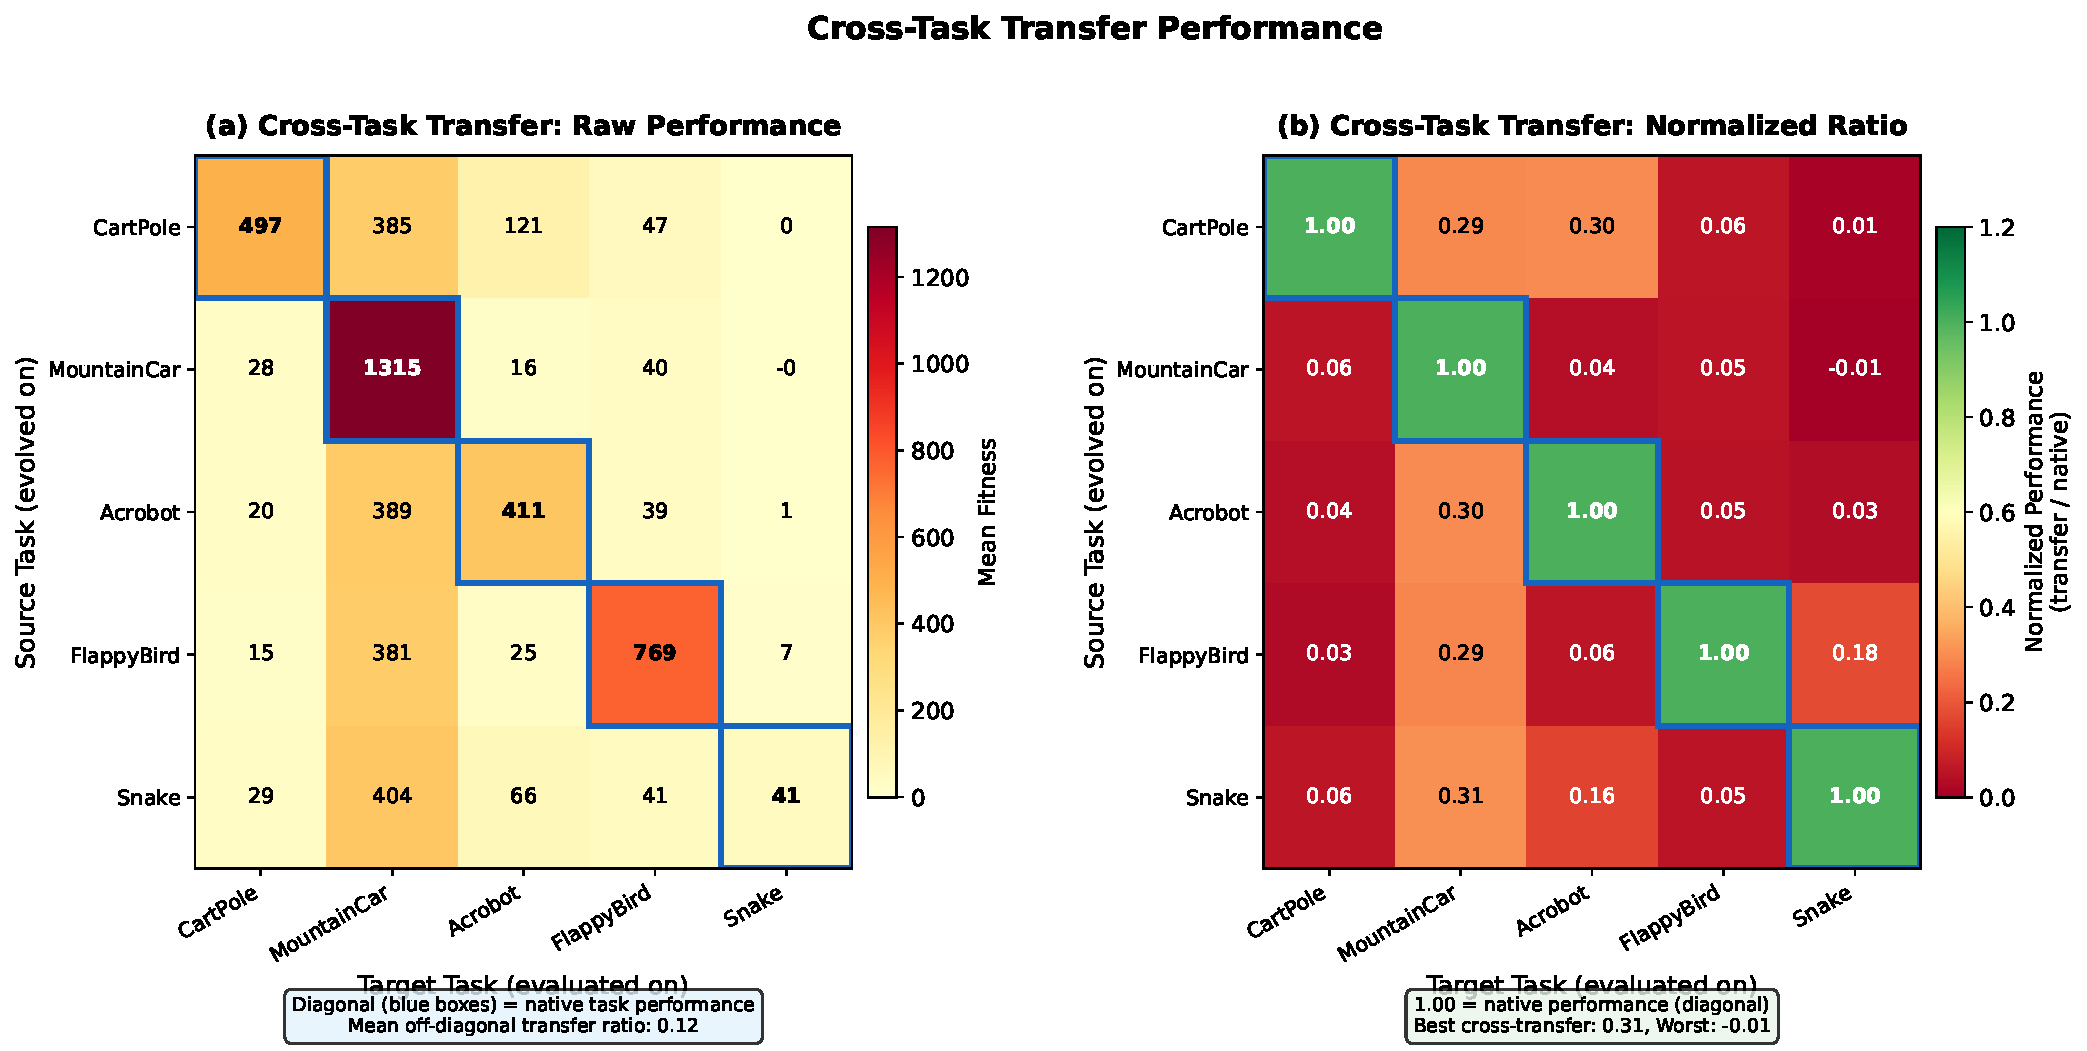
\includegraphics[width=\textwidth]{figures_arxiv/fig10_cross_task.pdf}
\caption{\textbf{Cross-task transfer performance.} (a)~Raw performance heatmap: mean fitness when the topology evolved on the source task configuration (rows) is embedded into and evaluated on the target task configuration (columns). Diagonal entries (blue boxes) show native task performance: CartPole~497, MountainCar~1{,}315, Acrobot~411, FlappyBird~769, Snake~41. Mean off-diagonal transfer: 0.12; best cross-transfer: 0.31. (b)~Normalized ratio heatmap: transfer fitness divided by native fitness. Diagonal is 1.00 by definition; off-diagonal values quantify cross-configuration reuse under the embedding protocol.}
\label{fig:cross_task}
\end{figure}

\begin{figure}[htbp]
\centering
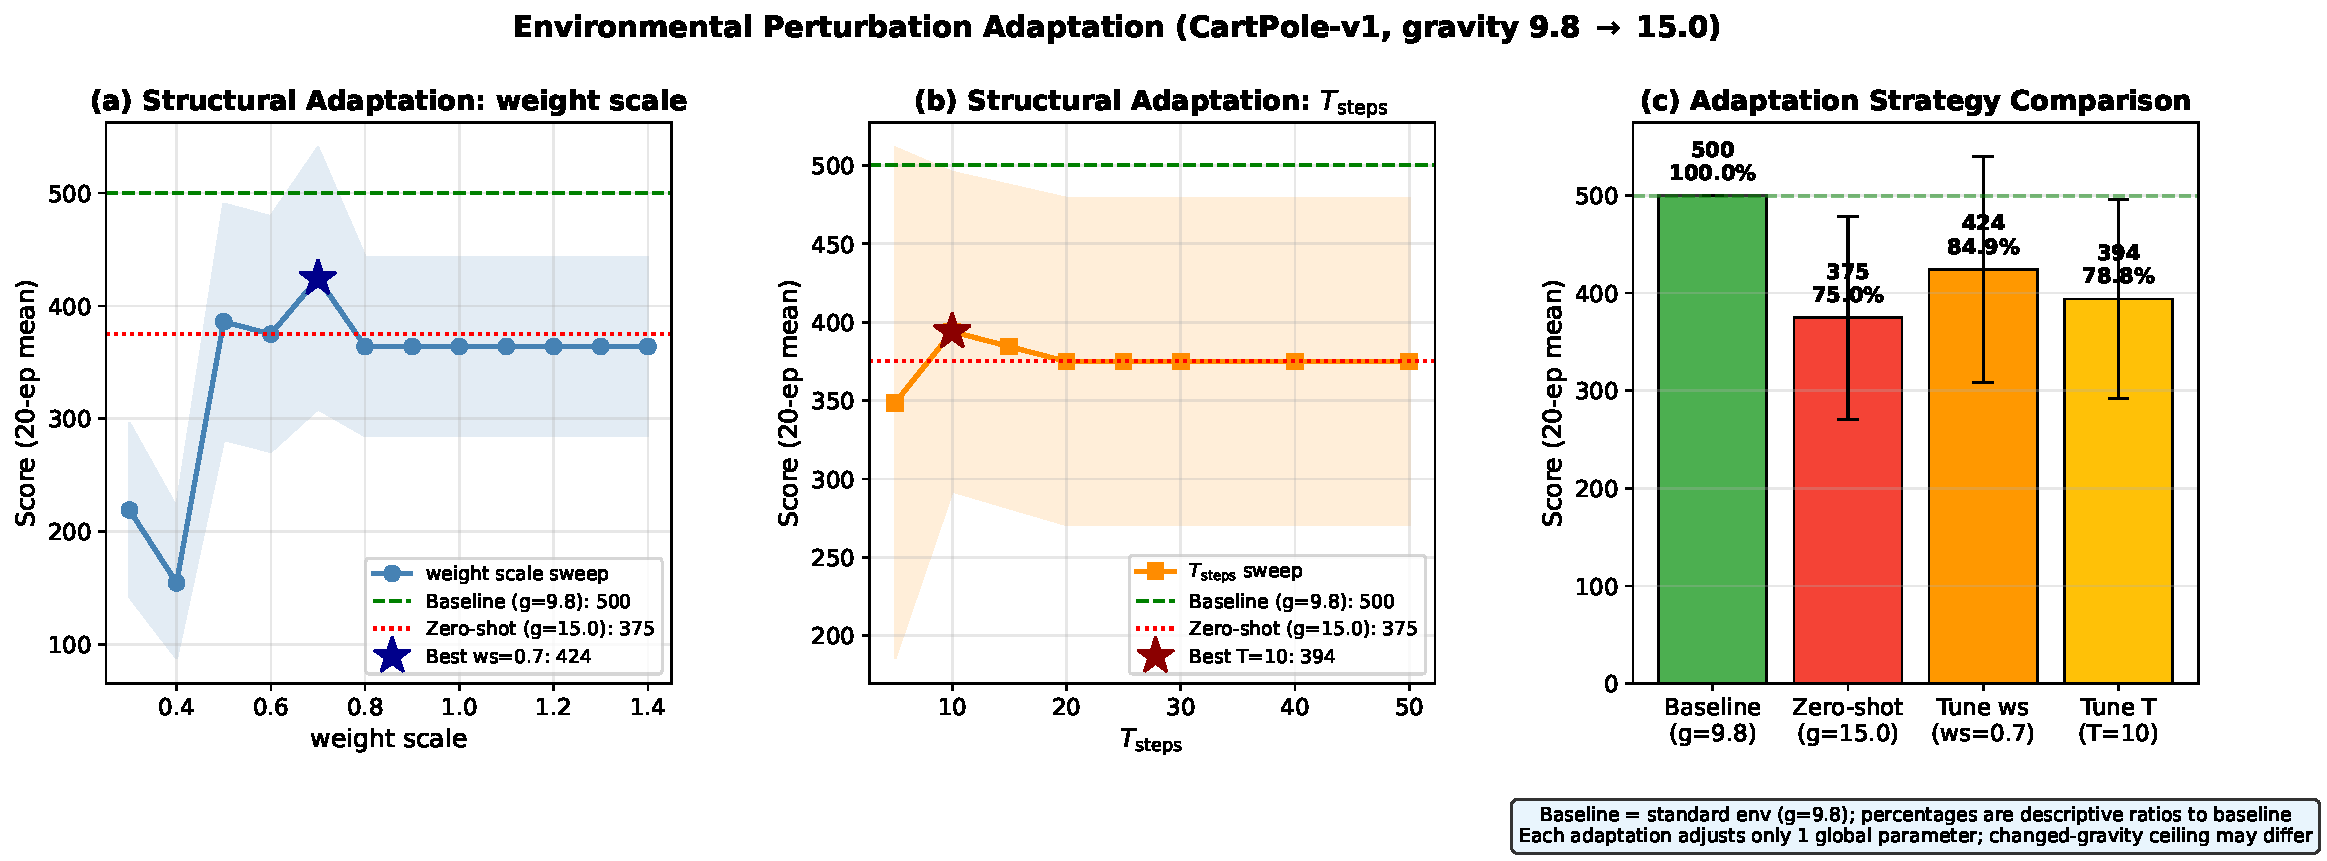
\includegraphics[width=\textwidth]{figures_arxiv/fig09_adaptation.pdf}
\caption{\textbf{Comparison of low-dimensional adaptation strategies to abrupt environmental change.} CartPole gravity is raised from 9.8 to 15.0. Panel (a) sweeps the single global weight scale; panel (b) sweeps $T_\text{steps}$; panel (c) summarizes the four evaluated settings. Baseline at standard gravity is $500$; zero-shot performance at gravity 15.0 is $375$; retuning $\mathit{weight\_scale}$ reaches $424$; retuning $T_\text{steps}$ reaches $394$. Dashed lines mark the standard-gravity and zero-shot references; error bars indicate episode-level evaluation variability.}
\label{fig:adaptation}
\end{figure}

\section{Discussion}

The main result is that binary recurrent topology, under fixed per-synapse
weights and a fixed global scale, can support reactive control in the tested
settings where weights would normally be optimized. On CartPole, topology-only
evolution does not produce a detectable performance loss relative to controls
that co-evolve weights, although this is a ceiling-bound result; on MountainCar,
it shows no statistically resolved disadvantage and no lower observed upper
range in our sample, but with a wide uncertainty interval. On LunarLander, a
higher-headroom reactive audit, topology-only evolution is not systematically
below independent-weight co-evolution, but the pre-specified 10\% TOST
equivalence margin is not supported. In a separate CartPole positioning audit,
it reaches the same ceiling regime as NEAT and PPO while using no independently
tuned per-synapse weights, though with slower convergence. The weight comparison
is therefore a bounded, task- and margin-dependent no-systematic-disadvantage
result, not a general equivalence claim.
Several converging analyses further indicate that, when such a fixed-weight
network succeeds, control performance depends on, and is most consistent with,
multi-step temporal iterative propagation through the evolved graph rather than
local connection motifs or precise hidden membrane values alone. This engineering result is
compatible with connectome-inspired observations---the compact fixed connectome
of \textit{C.\ elegans} \citep{white1986,cook2019,varshney2011}, structured
circuits in the \textit{Drosophila} mushroom body
\citep{eichler2017,scheffer2020}, and the view that behavioral complexity is not
captured by neuron count alone \citep{striedter2005,cisek2019}. We do not claim
that biological circuits use this mechanism; we show only that
structure--function coupling is plausible under conditions that remove
independently tunable per-synapse weights, and we restrict the claim to
reactive control and short-timescale temporal integration.

\subsection{Mechanism: temporal propagation as integration}

The picture supported by our experiments is that an evolved fixed-weight recurrent
topology propagates and mixes input signals over time, achieving temporal
integration through the global organization of its evolved paths rather than
through the enrichment of specific local motifs (Section~\ref{sec:exp-ablation}).
The number of internal propagation steps sets the integration window
($T_\text{steps}=1$ sharply reduces performance; reactive tasks saturate at a
shorter $T_\text{steps}$ than integrative ones), and the resulting trace is
behaviorally relevant: recent input history is linearly decodable from hidden
activity over a task-matched window, and output spike timing is systematically
modulated by velocity history in a near-upright subset of states
(Section~\ref{sec:exp-mechanism}). Consistently, resetting intermediate membrane
potentials does not substantially impair function, indicating that what matters is the
propagation path permitted by the connection structure more than a precise
instantaneous membrane vector. The non-spiking rate-substitution control further shows that
the evolved CartPole policy is not reproduced by simply replacing thresholded
spikes with a smooth iterated rate update. Finally, topology is calibrated to the
global weight scale used during evolution: changing that scale post hoc degrades
function unless the change is part of an explicit adaptation retuning, and
changing $T_\text{steps}$ alone does not generally restore it. Across five task
configurations, the resulting topologies carry configuration-identifiable
structure (leave-one-out KNN $94.0\%$), but architecture metadata alone are also
diagnostic in this data set and residualizing those metadata lowers the
structural classifier to $48.0\%$ (Section~\ref{sec:exp-fingerprint}).

\subsection{Relation to memory frameworks}

Recurrent-network memory models can be arranged along a state-versus-process axis,
and our result occupies a distinct position on it.
\begin{itemize}
\item \textbf{Attractor networks} \citep{hopfield1982,amit1989,amari1977} hold
memory as a stable fixed point---memory as an equilibrium \emph{state}, maintained
against perturbation, with partial biological support from engram studies
\citep{tonegawa2015,josselyn2020,liu2012}.
\item \textbf{Reservoir computing and liquid state machines}
\citep{jaeger2001,maass2002,lukosevicius2009,tanaka2019} hold memory as a
high-dimensional transient trajectory---memory as an ongoing \emph{process}, the
position closest to ours. The differences are that the reservoir topology is
typically random or hand-designed, whereas ours is evolved to the task, and that
reservoir computing still trains a readout, whereas we remove that degree of
freedom by using fixed output decoding rather than learned readout weights.
\item \textbf{Gated recurrent networks} (LSTM, GRU; \citealp{hochreiter1997,cho2014})
combine a persistent cell state with learned gates, so their memory rests on a
precisely learned continuous weight configuration rather than on structure.
\end{itemize}
Within this lineage, the present mechanism carries short-timescale history
through signal propagation along task-evolved fixed connection paths: it does
not rely on a stable attractor (LIF leakage, $\tau=5$~ms, makes persistent
storage nontrivial, and fixed-delay memory tasks fail), it depends on the
connection structure rather than on state values or gating, it is
robust to intermediate state perturbation (Section~\ref{sec:exp-mechanism}), and
its paths are shaped by the task rather than randomly projected
(Section~\ref{sec:exp-fingerprint}), while the current fingerprint evidence is
configuration-specific rather than architecture-independent.

\subsection{Implications and limitations}

Because no weight update is required during operation, the approach is
compatible with constraints that motivate neuromorphic hardware
\citep{davies2018,roy2019,schuman2017}: fixed weights remove the need for
on-chip learning circuitry, and the spiking implementation is compatible with
event-based sensing \citep{paredes2020}. The rate-substitution failure on the
same topology supports keeping the spiking dynamics in the present design, but
it does not by itself establish a hardware advantage or rule out rate networks
that are evolved from scratch. The practical implication is therefore modest: a
controller defined by a single global continuous scale, with its discrete
topology specified offline, may be useful on resource-constrained platforms if
future work verifies the energy and implementation benefits directly.

Several limitations bound these claims. (i) \emph{Fixed inductive biases.} The
E/I scaffold, global scale, output readout, LIF constants, and
$T_\text{steps}$ schedule are fixed design choices. We do not claim that topology
functions independently of these choices; rather, we claim that once they are
held fixed, searching only the topology can find reactive controllers in the
tested regime. (ii) \emph{Equivalence and benchmark difficulty.} CartPole is
ceiling-bound, and MountainCar has high seed-level variance. The LunarLander
headroom audit addresses the ceiling concern directly, but it does not convert
the comparison into a broad equivalence claim: TO is not systematically below TI
in that sample, while the uncertainty interval is too wide for the
pre-specified 10\% equivalence margin. The reported TOST sensitivity therefore
supports only explicitly stated, task-dependent margins rather than unrestricted
equivalence.
(iii) \emph{Mechanism evidence.} The $T_\text{steps}$ ablation changes both
internal propagation and output-spike accumulation opportunity, and the
spike-timing history analysis matches pole angle but not all CartPole state
dimensions. Stronger causal isolation will require controls that preserve output
opportunity while perturbing recurrent paths and paired analyses that match all
current-state dimensions. (iv) \emph{Spiking versus rate dynamics.} The rate-substitution control rules
out a simple post hoc rate replacement on the evolved topology, but not a
separately evolved non-spiking rate controller. (v) \emph{Structural
fingerprints.} Cross-task fingerprints are confounded by task-specific network
size and I/O dimensions, so they identify configurations rather than an
architecture-independent task metric. (vi) \emph{Scale and action dimensionality.}
The networks are small
($64$--$128$ neurons), and the method does not reach proficiency on
higher-dimensional action spaces (Section~\ref{sec:exp-boundary}); the likely
limiting factor is that multi-joint coordination grows combinatorially and
exceeds what a single global scale can express, so crossing this boundary
probably requires structural innovation (for example, modular or per-output
sub-topologies) and improvements to the search itself, since local bit-flip
mutation explores the $2^{N^2}$ space only locally. (vii)
\emph{Single-topology continuous control.} The continuous-control results come
from one evolved topology (seed~42) evaluated over episodes, so they are a
proof-of-concept rather than a multi-seed benchmark like the discrete tasks. (viii)
\emph{Working memory and transfer.} The fixed-weight network fails on fixed-delay
discrete-memory tasks ($23$--$54\%$, near chance) and does not transfer zero-shot
across task configurations under our embedding protocol, consistent with
task-specialized recurrent paths and with the absence of stable attractor states
under LIF leakage. (ix) \emph{Noisy-fitness overfitting.} Sparse fitness evaluation
inflates the generalization gap (28.9\% at 3 episodes versus 3.4\% at 8), a known
property of evolutionary search under noisy fitness
\citep{rechenberg1973,fogel1995} that denser or multi-objective evaluation may
reduce.

\section{Conclusion}

We asked whether a binary recurrent connection topology, evaluated under fixed
dynamics and a task-specified global weight scale, can support reactive control
once per-synapse weight learning is removed. On CartPole, under an aligned
control protocol, evolving only the binary adjacency matrix did not produce a
detectable performance loss relative to co-evolving per-synapse weights, but
this result is ceiling-bound and should not be read as unrestricted equivalence;
on MountainCar, the same comparison showed no statistically resolved
disadvantage and no lower observed upper range in our sample, but with a wide
uncertainty interval. On LunarLander, a higher-headroom audit, the
topology-only condition was not systematically below independent weight
co-evolution, but the pre-specified 10\% TOST equivalence margin was not
supported. In a separate CartPole positioning audit, the method reached the same
ceiling regime as NEAT and PPO, although not with the same convergence speed.
When such networks succeed, converging but not fully causal evidence---the
$T_\text{steps}$ ablation, history decoding, intermediate-state perturbation,
history-dependent spike timing, and the failure of a post hoc rate-substitution
control---points to temporal iterative propagation through the evolved graph as
a plausible mechanism. Evolved topologies carry configuration-identifiable
structure, but that analysis is substantially confounded by architecture
metadata. The approach extends to low-dimensional continuous locomotion as a
single-topology proof-of-concept and adapts to a tested abrupt environmental
change by retuning one global parameter. It is bounded, in its present form, by
discrete working memory, zero-shot transfer, architecture-confounded structural
fingerprints, and higher-dimensional action spaces. Taken together, these
results provide evidence that, for reactive control and short-timescale temporal
integration, connection structure together with a compatible global dynamical
scale can support control policies in these benchmark settings, while also
indicating the limits of this regime. Whether the same principle extends to
higher-performance headroom tasks, higher-dimensional control, and tasks
requiring persistent memory---through larger or modular networks and improved
structural search---is, we suggest, a question worth pursuing.

\section*{Author contributions}
Xuewei Li proposed the research conception and theoretical framework, designed the experimental scheme, and wrote the manuscript. Bowen Zhao implemented the experimental system, carried out all experiments, and revised and validated the experimental design. Guangxu Mei participated in research discussions and methodological refinement. All authors reviewed and approved the final manuscript. Xuewei Li and Bowen Zhao contributed equally as co-first authors.

\section*{Code and data availability}
The implementation, experimental scripts, configuration files, random seeds,
processed result files, and figure-generation scripts are available in the public
repository at
\url{https://github.com/xuewei1413/recurrent_topology_supports_reactive_control}.
The archival snapshot used for this manuscript is tagged
\texttt{v1.0-submission-artifact}. The local submission artifact includes
seed-level TO/TG/TI result tables, a manifest, and scripts that regenerate the
confidence-interval, TOST-sensitivity, and availability-audit summaries reported
above. Large raw logs, local cluster launch scripts, third-party tools, and
duplicate legacy result folders are not part of the archival artifact; raw logs
not included in the repository or supplementary archive will be made available by
the corresponding author upon reasonable request.

\begin{thebibliography}{99}

\bibitem[Amari(1977)]{amari1977}
Amari, S.-I. (1977). Dynamics of pattern formation in lateral-inhibition type neural fields. \textit{Biological Cybernetics}, 27(2), 77--87.
\bibitem[Anwar(2021)]{anwar2021}
Anwar, A. (2021). Evolving spiking circuit motifs using weight agnostic neural networks. \textit{Proceedings of the AAAI Conference on Artificial Intelligence}, 35(14), 12447--12455.
\bibitem[Amit(1989)]{amit1989}
Amit, D.~J. (1989). \textit{Modeling Brain Function: The World of Attractor Neural Networks}. Cambridge University Press.
\bibitem[Cho et~al.(2014)]{cho2014}
Cho, K., van Merri\"{e}nboer, B., Gulcehre, C., et~al. (2014). Learning phrase representations using RNN encoder-decoder for statistical machine translation. \textit{EMNLP}.
\bibitem[Cisek(2019)]{cisek2019}
Cisek, P. (2019). Resynthesizing behavior through phylogenetic refinement. \textit{Attention, Perception, \& Psychophysics}, 81(7), 2265--2287.
\bibitem[Cook et~al.(2019)]{cook2019}
Cook, S.~J., Jarrell, T.~A., Brittin, C.~A., et~al. (2019). Whole-animal connectomes of both \textit{Caenorhabditis elegans} sexes. \textit{Nature}, 571(7763), 63--71.
\bibitem[Davies et~al.(2018)]{davies2018}
Davies, M., Srinivasa, N., Lin, T.-H., et~al. (2018). Loihi: A neuromorphic manycore processor with on-chip learning. \textit{IEEE Micro}, 38(1), 82--99.
\bibitem[Dorkenwald et~al.(2024)]{dorkenwald2024}
Dorkenwald, S., Matsliah, A., Sterling, A.~R., et~al. (2024). Neuronal wiring diagram of an adult brain. \textit{Nature}, 634(8032), 124--138.
\bibitem[Eccles(1976)]{eccles1976}
Eccles, J.~C. (1976). From electrical to chemical transmission in the central nervous system. \textit{Notes and Records of the Royal Society of London}, 30(2), 219--230.
\bibitem[Eiben and Smith(2015)]{eiben2015}
Eiben, A.~E., \& Smith, J.~E. (2015). \textit{Introduction to Evolutionary Computing} (2nd ed.). Springer.
\bibitem[Eichler et~al.(2017)]{eichler2017}
Eichler, K., Li, F., Litwin-Kumar, A., et~al. (2017). The complete connectome of a learning and memory centre in an insect brain. \textit{Nature}, 548(7666), 175--182.
\bibitem[Fogel(1995)]{fogel1995}
Fogel, D.~B. (1995). \textit{Evolutionary Computation: Toward a New Philosophy of Machine Intelligence}. IEEE Press.
\bibitem[Frankle and Carbin(2019)]{frankle2019}
Frankle, J., \& Carbin, M. (2019). The lottery ticket hypothesis: Finding sparse, trainable neural networks. \textit{ICLR}.
\bibitem[Frankle et~al.(2020)]{frankle2020}
Frankle, J., Dziugaite, G.~K., Roy, D.~M., \& Carbin, M. (2020). Linear mode connectivity and the lottery ticket hypothesis. \textit{ICML}.
\bibitem[Gaier and Ha(2019)]{gaier2019}
Gaier, A., \& Ha, D. (2019). Weight agnostic neural networks. \textit{Advances in Neural Information Processing Systems}, 32.
\bibitem[Gerstner et~al.(2014)]{gerstner2014}
Gerstner, W., Kistler, W.~M., Naud, R., \& Paninski, L. (2014). \textit{Neuronal Dynamics: From Single Neurons to Networks and Models of Cognition}. Cambridge University Press.
\bibitem[Harris and Shepherd(2015)]{harris2015}
Harris, K.~D., \& Shepherd, G.~M. (2015). The neocortical circuit: Themes and variations. \textit{Nature Neuroscience}, 18(2), 170--181.
\bibitem[Hochreiter and Schmidhuber(1997)]{hochreiter1997}
Hochreiter, S., \& Schmidhuber, J. (1997). Long short-term memory. \textit{Neural Computation}, 9(8), 1735--1780.
\bibitem[Holland(1992)]{holland1992}
Holland, J.~H. (1992). \textit{Adaptation in Natural and Artificial Systems}. MIT Press.
\bibitem[Hopfield(1982)]{hopfield1982}
Hopfield, J.~J. (1982). Neural networks and physical systems with emergent collective computational abilities. \textit{Proceedings of the National Academy of Sciences}, 79(8), 2554--2558.
\bibitem[Jaeger(2001)]{jaeger2001}
Jaeger, H. (2001). The ``echo state'' approach to analysing and training recurrent neural networks. \textit{GMD Report}, 148, German National Research Center for Information Technology.
\bibitem[Jin et~al.(2026)]{jin2026}
Jin, Z., Zhu, Y., Zhang, C., \& Sui, Y. (2026). Whole-brain connectomic graph model enables whole-body locomotion control in fruit fly. \textit{arXiv preprint}, arXiv:2602.17997. https://doi.org/10.48550/arXiv.2602.17997.

\bibitem[Josselyn and Tonegawa(2020)]{josselyn2020}
Josselyn, S.~A., \& Tonegawa, S. (2020). Memory engrams: Recalling the past and imagining the future. \textit{Science}, 367(6473), eaaw4325.
\bibitem[Liu et~al.(2012)]{liu2012}
Liu, X., Ramirez, S., Pang, P.~T., et~al. (2012). Optogenetic stimulation of a hippocampal engram activates fear memory recall. \textit{Nature}, 484(7394), 381--385.
\bibitem[Luko\v{s}evi\v{c}ius and Jaeger(2009)]{lukosevicius2009}
Luko\v{s}evi\v{c}ius, M., \& Jaeger, H. (2009). Reservoir computing approaches to recurrent neural network training. \textit{Computer Science Review}, 3(3), 127--149.
\bibitem[Maass et~al.(2002)]{maass2002}
Maass, W., Natschl\"{a}ger, T., \& Markram, H. (2002). Real-time computing without stable states: A new framework for neural computation based on perturbations. \textit{Neural Computation}, 14(11), 2531--2560.
\bibitem[Maass(1997)]{maass1997}
Maass, W. (1997). Networks of spiking neurons: The third generation of neural network models. \textit{Neural Networks}, 10(9), 1659--1671.
\bibitem[Markram et~al.(2004)]{markram2004}
Markram, H., Toledo-Rodriguez, M., Wang, Y., Gupta, A., Silberberg, G., \& Wu, C. (2004). Interneurons of the neocortical inhibitory system. \textit{Nature Reviews Neuroscience}, 5(10), 793--807.
\bibitem[Milo et~al.(2002)]{milo2002}
Milo, R., Shen-Orr, S., Itzkovitz, S., Kashtan, N., Chklovskii, D., \& Alon, U. (2002). Network motifs: Simple building blocks of complex networks. \textit{Science}, 298(5594), 824--827.
\bibitem[Paredes-Vall\'{e}s et~al.(2020)]{paredes2020}
Paredes-Vall\'{e}s, F., Scheper, K.~Y.~W., \& de Croon, G.~C.~H.~E. (2020). Unsupervised learning of a hierarchical spiking neural network for optical flow estimation: From events to global motion perception. \textit{IEEE Transactions on Pattern Analysis and Machine Intelligence}, 42(8), 2051--2064.
\bibitem[Ramanujan et~al.(2020)]{ramanujan2020}
Ramanujan, V., Wortsman, M., Kembhavi, A., Farhadi, A., \& Rastegari, M. (2020). What's hidden in a randomly weighted neural network? \textit{CVPR}.
\bibitem[Rechenberg(1973)]{rechenberg1973}
Rechenberg, I. (1973). \textit{Evolutionsstrategie: Optimierung technischer Systeme nach Prinzipien der biologischen Evolution}. Frommann-Holzboog.
\bibitem[Roy et~al.(2019)]{roy2019}
Roy, K., Jaiswal, A., \& Panda, P. (2019). Towards spike-based machine intelligence with neuromorphic computing. \textit{Nature}, 575(7784), 607--617.
\bibitem[Scheffer et~al.(2020)]{scheffer2020}
Scheffer, L.~K., Xu, C.~S., Januszewski, M., et~al. (2020). A connectome and analysis of the adult \textit{Drosophila} central brain. \textit{eLife}, 9, e57443.
\bibitem[Schulman et~al.(2017)]{schulman2017}
Schulman, J., Wolski, F., Dhariwal, P., Radford, A., \& Klimov, O. (2017). Proximal policy optimization algorithms. \textit{arXiv preprint}, arXiv:1707.06347.
\bibitem[Schuman et~al.(2017)]{schuman2017}
Schuman, C.~D., Potok, T.~E., Patton, R.~M., Birdwell, J.~D., Dean, M.~E., Rose, G.~S., \& Plank, J.~S. (2017). A survey of neuromorphic computing and neural networks in hardware. \textit{arXiv preprint}, arXiv:1705.06963.
\bibitem[Stanley and Miikkulainen(2002)]{stanley2002}
Stanley, K.~O., \& Miikkulainen, R. (2002). Evolving neural networks through augmenting topologies. \textit{Evolutionary Computation}, 10(2), 99--127.
\bibitem[Stanley et~al.(2009)]{stanley2009}
Stanley, K.~O., D'Ambrosio, D.~B., \& Gauci, J. (2009). A hypercube-based encoding for evolving large-scale neural networks. \textit{Artificial Life}, 15(2), 185--212.
\bibitem[Strata and Harvey(1999)]{strata1999}
Strata, P., \& Harvey, R. (1999). Dale's principle. \textit{Brain Research Bulletin}, 50(5--6), 349--350.
\bibitem[Striedter(2005)]{striedter2005}
Striedter, G.~F. (2005). \textit{Principles of Brain Evolution}. Sinauer Associates.
\bibitem[Tanaka et~al.(2019)]{tanaka2019}
Tanaka, G., Yamane, T., H\'{e}roux, J.~B., Nakane, R., Kanazawa, N., Takeda, S., Numata, H., Nakano, D., \& Hirose, A. (2019). Recent advances in physical reservoir computing: A review. \textit{Neural Networks}, 115, 100--123.
\bibitem[Tonegawa et~al.(2015)]{tonegawa2015}
Tonegawa, S., Liu, X., Ramirez, S., \& Redondo, R. (2015). Memory engram cells have come of age. \textit{Neuron}, 87(5), 918--931.
\bibitem[Varshney et~al.(2011)]{varshney2011}
Varshney, L.~R., Chen, B.~L., Paniagua, E., Hall, D.~H., \& Chklovskii, D.~B. (2011). Structural properties of the \textit{Caenorhabditis elegans} neuronal network. \textit{PLOS Computational Biology}, 7(2), e1001066.
\bibitem[White et~al.(1986)]{white1986}
White, J.~G., Southgate, E., Thomson, J.~N., \& Brenner, S. (1986). The structure of the nervous system of the nematode \textit{Caenorhabditis elegans}. \textit{Philosophical Transactions of the Royal Society B}, 314(1165), 1--340.
\bibitem[Wang et~al.(2023)]{wang2023}
Wang, G., Sun, Y., Cheng, S., \& Song, S. (2023). Evolving connectivity for recurrent spiking neural networks. \textit{Advances in Neural Information Processing Systems}, 36.
\bibitem[Zhou et~al.(2019)]{zhou2019}
Zhou, H., Lan, J., Liu, R., \& Yosinski, J. (2019). Deconstructing lottery tickets: Zeros, signs, and the supermask. \textit{Advances in Neural Information Processing Systems}, 32.
\end{thebibliography}

\end{document}


